%Typeset using XeLaTeX

\documentclass[10pt,a4paper]{book}
\usepackage{mathtools,amssymb,amsthm}
%\usepackage{phonetic}
\usepackage{fancyhdr}
\usepackage[pass]{geometry}
\usepackage{fontspec}
%\usepackage{xunicode}
%\usepackage{xltxtra}
%\usepackage{xgreek}
\setmainfont[Mapping=TeX-text]{Times New Roman}
\usepackage{hyperref}
%\usepackage{color}
\usepackage[Glenn]{fncychap}
\ChNameVar{\bfseries\Large}
%\usepackage{tabularx}
%\usepackage[normalem]{ulem}

\usepackage{enumerate}
\usepackage{tikz}
\usepackage{multicol}
\usepackage{natbib}

\renewcommand{\maketitle}{
	\begin{titlepage}
		\newgeometry{left=4cm, top=2.3cm, bottom=2.3cm}
		\hbox{\mbox{\hspace{-1.3cm}}
			\vrule depth 0.98\textheight
			\mbox{\hspace{1cm}}
			\vtop{
				\vspace{2cm}
				\begin{flushleft}
					\huge{\bf Pricing Games in Heterogeneous Parallel Networks\\}
					\vskip3cm
					\Large  Thomas Pappas\\
					AL1.18.0011\\
					\vskip3cm
					\begin{minipage}{7.5cm}
						\begin{flushleft}
							\normalsize {\it {\bf Examination committee:}\\
								Dimitris Fotakis, School of Electrical and Computer Engineering, National Technical University of Athens.\\
								Professor's name, Department or School, Institution.\\
								Professor's name, Department or School, Institution.}
						\end{flushleft}
					\end{minipage}
					\hskip0.5cm
					\begin{minipage}{6cm}
						\begin{flushleft}
							\normalsize {\it {\bf Supervisor:}\\
								Dimitris Fotakis, Professor, \\ School of Electrical and Computer Engineering,\\
								National Technical University of Athens.\\
							}
						\end{flushleft}
					\end{minipage}
				\end{flushleft}
				\vskip6cm
				\hskip4.5cm
				\begin{minipage}{5cm}
					\begin{center}
						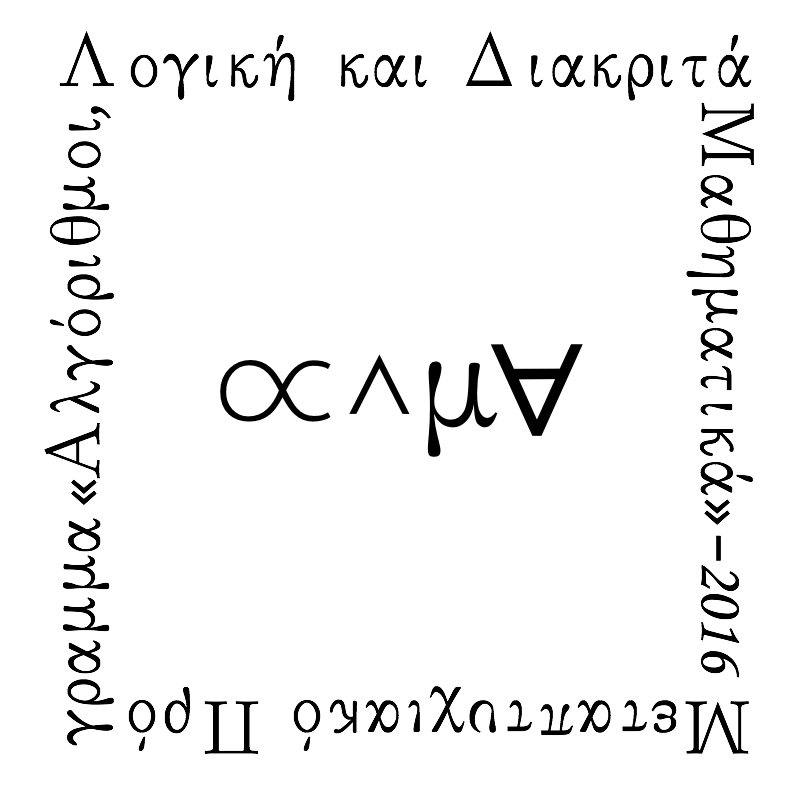
\includegraphics[width=0.8\textwidth]{alma.png}
					\end{center}
		\end{minipage}}}
	\end{titlepage}
}

% Commands for wrapping properly common expressions.
\newcommand{\indeq}[1]{\stackrel{\text{#1}}{=}}
\newcommand{\RightarrowArg}[1]{\stackrel{#1}{\Rightarrow}}
\newcommand{\LeftrightarrowArg}[1]{\stackrel{#1}{\Leftrightarrow}}
\newcommand{\NE}{\mathrm{N.E.}}
\newcommand{\as}{\mathrm{\alpha_s}}
\newcommand{\R}{\mathbb{R}}
\newcommand{\Gm}{\mathcal{G}}
\DeclareMathOperator*{\argmax}{arg\,max}
% \newcommand{\Exp}{\mathrm{Exp}}
% \newcommand{\Expect}{{\rm I\kern-.3em E}}

% Theorem structures.
\theoremstyle{definition}
\newtheorem{ex}{}[section]
\newtheorem{definition}{Definition}[chapter]
\newtheorem{theorem}[definition]{Theorem}
\newtheorem{lemma}[definition]{Lemma}
\newtheorem{corollary}[definition]{Corollary}
\theoremstyle{comment}
\newtheorem{example}[definition]{Example}
\newtheorem{claim}[definition]{Claim}

\fancyhead[LO]{\slshape \leftmark}
\fancyhead[RE]{\slshape \rightmark}
\fancyhead[LE]{}
\fancyhead[RO]{}
\fancyfoot[LO,RE]{\tiny{\it}}

% Main document
\begin{document}

\maketitle
\clearpage


\thispagestyle{empty}
\null
\clearpage

\restoregeometry

\thispagestyle{empty}
\pagenumbering{gobble}
\chapter*{Abstract}
In this masters thesis we study a $2$-level optimisation problem where, on an $n$-link network from a source $s$ to a target $t$, a unit of flow wants to move from $s$ to $t$ using the link with the lowest cost, while the link owners compete for profit by assigning tolls to links and thus creating a toll congestion game.
We examine only affine latencies for the links.
In addition, each flow player responds to tolls in a heterogeneous way, i.e. each flow player $p$ has a different money-time sensitivity value, which is described by a distribution function $\alpha(p)$.
First we present some basic definitions and properties of profit homogeneous games.
Using them as base, we examine cases of fixed and step distribution functions, where for the latter we first restrict our model to $2$-link instances and then we present strict conditions for the existence or not of a Nash Equilibrium.
We then introduce a new term, the split function $\as(t)$, defined as the time-money sensitivity value for which the $2$ link costs are equal for a given set of tolls $t$. With the help of $\as$ we will describe and prove some properties of the heterogeneous games for continuous distribution functions.
In our main result, we generalise the conditions necessary for the existence of a Nash Equilibrium in the profit game between two toll owners, and finally we discuss some extensions to $n$-link parallel networks.
\clearpage

\thispagestyle{empty}
\null
\clearpage

\thispagestyle{empty}
\pagenumbering{gobble}
\chapter*{Συνοψη}
Σε αυτή τη διπλωματική μεταπτυχιακού μελετάμε ένα πρόβλημα βελτιστοποίησης $2$ επιπέδων, όπου σε ένα δίκτυο με $n$ ακμές από μια πηγή $s$ σε ένα στόχο $t$, μια μονάδα ροής θέλει να μετακινηθεί από το $s$ στο $t$ χρησιμοποιώντας την ακμή με το χαμηλότερο κόστος, ενώ οι δύο ιδιοκτήτες των ακμών ανταγωνίζονται για κέρδος βάζοντας δίοδια στις ακμές και δημιουργώντας έτσι ένα παίγνιο συμφόρησης με διόδια.
Εξετάζουμε μόνο αφινικές καθυστερήσεις για τις ακμές.
Επιπλέον, ο κάθε παίκτης ροής αντιδρά στα διόδια με ετερογενή τρόπο, δηλ. ο κάθε παίκτης ροής $p$ έχει διαφορετική τιμή ευαισθησίας χρόνου-χρήματος, η οποία περιγράφεται από μια συνάρτηση κατανομής $\alpha(p)$.
Πρώτα παρουσιάζουμε κάποιους βασικούς ορισμούς και ιδιότητες των ομογενών παιγνίων κέρδους.
Mε αυτά ως βάση, εξετάζουμε περιπτώσεις σταθερών και βηματικών συναρτήσεων κατανομής, όπου για το τελευταίο πρώτα περιοριζόμαστε σε στιγμιότυπα $2$ ακμών και παρουσιάζουμε αυστηρές συνθήκες για την ύπαρξη ή μη σημείου ισορροπίας Nash.
Μετά εισαγάγουμε έναν νέο όρο, τη συνάρτηση διαχωρισμού $\as(t)$, ορισμένη ως η τιμή ευαισθησίας χρόνου-χρήματος για την οποία τα κόστη των $2$ ακμών είναι ίσα για ένα δοσμένο σετ διοδίων $t$.
Με τη βοήθεια της $\as$ θα περιγράψουμε και θα αποδείξουμε μερικές ιδιότητες των ετερογενών παιγνίων με συνεχή συνάρτηση κατανομής.
Στο κύριο αποτέλεσμά μας, γενικοποιούμε τις συνθήκες που είναι απαραίτητες για την ύπαρξη ισορροπίας Nash στο παίγνιο κέρδους μεταξύ δύο ιδιοκτητών ακμών, και τελικώς συζητάμε κάποιες επεκτάσεις για δίκτυα με $n$ ακμές.
\clearpage

\thispagestyle{empty}
\null
\clearpage

\pagestyle{fancy}

\pagenumbering{roman}
\tableofcontents
\clearpage

\thispagestyle{empty}
\null
\clearpage

\pagenumbering{arabic}


\chapter{Introduction}
\label{chapter:intro}

In this thesis we study a two level optimisation problem.
On the basis there is a network with 2 nodes $(s, t)$ and $n$ links, each link directed from $s$ to $t$ and weighted by a non-decreasing latency function that defines how the traffic increases as more players flow into that link.
On the first level, a flow $[0, 1]$ wants to move from $s$ to $t$ using one of the $n$ links and experience minimum latency (traffic).
On the second level, each link is owned by a different owner who can add a toll to their link and gain profit proportional to the flow that uses it.
The tolls impose an additional cost to the flow players, affecting the first level game, and the link owners compete with each other to maximise their profit.
In our case we will additionally assume that the flow users behave in a heterogeneous way when it comes to tolls, meaning that each player has a different money-time trade-off and thus see the link costs differently.

The structure of this thesis is as such.
We finish this chapter by briefly presenting previous work in this field, all while examining some of the different models and properties that have been researched in the literature so far.
This will also serve as a bridge to Chapter \ref{chapter:preliminaries} were we will set our basis for the rest of the study.
This includes formal definitions of the models and properties we introduced from previous work as well as some additional -but still basic- properties of the models, with heavy focus on the money-time user sensitivity, captured by a distribution function $\alpha$.

Entering the main body of our work, in Chapter \ref{chapter:split} we introduce a new term regarding any two links of the network, called \textit{money-time sensitivity split}, which captures the notion of a (potentially non-existent) player whose money-time sensitivity makes them view the two links as equal.
We will then analyse that notion and provide properties and bounds for its values.
Finally, in the chapter's main result, we prove a general property of homogeneous network games as, due to the previously found bounds, there might be a portion of users whose sensitivity value can be arbitrarily large without affecting the game.

Having arrived at our main results in this work, in Chapter \ref{chapter:pricing_equilibria} we investigate the pricing competition game between the link owners of a network with heterogeneous users.
We begin by examining a class of games where the distribution function is fixed across all users, which, as we'll formally describe, makes the game \textit{pseudo-heterogeneous}.
Particular interest in the above class is the relation between games with identical setup but with different fixed distribution functions.
We describe and prove some properties for them, and using those we then tackle step distribution functions (where the user sensitivity can take values out of a finite set).
At this point we restrict our model to instances with $2$ links, and provide strict restrictions for equilibrium existence for the pricing competition game.

We conclude this thesis with a short discussion around the main outtakes of this study, while also presenting potential directions for future work.


\section{Related Work}
\label{section:related_work}

Selfish routing has a vast history of literature as it's been proven useful in solving a variety of real-world problems in economics \cite{pigou1920economics}, transportation \cite{beckmann1956studies} and more (see \cite{roughgarden2002sr} and \cite{roughgarden2005slpoa} for more references).
It has been well-established, at least as early as 1920 from the work of Pigou \cite{pigou1920economics}, that selfish behavior in congested networks can create (arbitrary) inefficiencies with regard to the total latency experienced by all users.
A long-standing practice to solve these inefficiencies has been to regulate the network by adding tolls to the links, thus altering the cost of the link usage.
A classical result on this is the use of marginal tolls (Beckman et al. \cite{beckmann1956studies}), where each link user is charged a toll corresponding to their externality, i.e. the added congestion effect caused by their participation in the network.
This technique can eradicate the inefficiencies and create optimal flow in the network, however it assumes a strong homogeneity among the users.
Marginal cost pricing has been investigated in networks with homogeneous users (e.g. Dafermos \cite{dafermos1973toll}), with the resulting payment required by users on same links being different, an unwanted and non-practical approach, which also requires knowledge of the users' sensitivity beforehand.

Congestion games were formally introduced by Rosenthal \cite{Rosenthal1973ACO} who also proved that in those games a pure Nash Equilibrium always exists.
Later, Monterer-Shapely \cite{MONDERER1996124} defined the class of potential games (games where the incentive for all players to change their strategy can be expressed with a global function) and proved that congestion games are equivalent to exact potential games (potential games where a change in strategy from any player alter the potential function the exact way it alters the player's cost).
One of the major contributions in this field has been the introduction of the Wardrop equilibrium \cite{wardrop_theoretical_1952}, a notion of Nash equilibrium for potential games, where the Wardrop principles provide a framework to describe and analyse those equilibria.
Milchtaich \cite{MILCHTAICH1996111} then investigated different pay-off functions for congestion games, where he showed that even though some best-reply strategies may end up in a cyclic path, there is always a path that leads to Nash equilibrium with pure strategies.

Given the above, with the existence of a Nash equilibrium always existing, later research focused on investigating the quality of an equilibrium by using the notion of \textit{Price of Anarchy}, introduced by Koutsoupias-Papadimitriou \cite{KOUTSOUPIAS200965}.
The Price of Anarchy describes the ratio between a Nash Equilibrium and the most cost-efficient solution, therefore lower values denote a qualitative equilibrium while a lower value denotes a bad one.
Finally, in terms of complexity, Fabrikant et al. \cite{10.1145/1007352.1007445} have shown that calculating a pure Nash Equilibrium for congestion games is PLS-complete in the general case.

Regarding the model properties, there is a multitude of variations in the classical selfish routing model.
Beginning with the network topology, one can distinguish between parallel networks (our case) or series-parallel ones.
In addition the flow traversing through the network can either be atomic (finite number of players, each contributing to congestion equally or weighted) or non-atomic (infinite number of players, each contributing to congestion by an non-influencing infinitesimal amount).
Also the model might admit elastic demand (e.g. \cite{10.1287/moor.1060.0231}, \cite{Hearn1998}), a property where the users have a bound on the cost they're willing to pay, making instances having potential players not participating in the flow.

Most work considers homogeneous network users.
Heterogeneity has been studied by Schmeilder \cite{1973JSP.....7..295S} and Milchtaich \cite[Prop 3.3]{doi:10.1287/moor.25.3.349.12220} has contributed through with work on the more general crowding games, a class of games where the cost assigned to each player is affected only by the number of players selecting the same action (or strategy).
Large crowding games are basically less restrictive $n$-link parallel congestion games.
Also, Cole et al. \cite{10.1145/780542.780618} in their work showed that even general heterogeneous networks can be priced so that an optimal routing emerges while computing those efficient tolls can be done in polynomial time for convex latency functions and distribution functions with only finitely many values.
The latter paper has been one of the main pillars of this thesis.

Discussing more the algorithmic aspect of toll computation, there has been significant research in finding optimal tolls for homogeneous network users.
Marginal cost prices can be computed using convex programming \cite{beckmann1956studies}, while the transportation community has made significant progress in optimising efficient computation and characterisating minimum-latency tolls (\cite{10.1007/978-3-642-59179-2_4}, \cite{Hearn1998}, \cite{Hearn2002}).

Acemoglu and Ozdaglar were the first to introduce pricing competition between link owners to the above model \cite{10.1287/moor.1060.0231}.
They showed that increasing the competition among operators from a monopoly to an oligopoly may reduce the efficiency of the network, achieving tight bounds on the Price of Anarchy.
In a follow-up work \cite{10.1109/JSAC.2007.070812}, they generalised the above by assuming more general topologies where links can also be linked serially (series-parallel networks).
Correa et al. \cite{correa2018pricing} showed pricing games may not exist, may not be unique and can be arbitrarily inefficient, but regulating the network with toll caps can solve all three issues.
Harkes et al. \cite{Harks_2019} then showed that the same is true for uniform toll caps, which is stronger in practice as toll discrimination is often not allowed.
The latter two papers have also been main pillars of the current work.


\cleardoublepage


\chapter{Preliminaries}
\label{chapter:preliminaries}

In this section we will describe the model utilised throughout this thesis.
If we attempted to call that model by including all of its properties, the result would be a Heterogeneous Non-atomic 2-link Parallel Network Toll Congestion Pricing Game, so while we will describe each of those properties, we will eventually focus on heterogeneity and the pricing competition, thus calling it a Heterogeneous Pricing Game.

\section*{Non-atomic Parallel Network Games}

We consider a directed graph $G = (\{s, t\}, N)$ where $N = \{1,\dots, n\}$ is a set of parallel links from a source node $s$ to a target node $t$.
For the non-atomic case, there is one unit of traffic that wishes to travel from $s$ to $t$, described as the unit interval $[0, 1]$ endowed with Lebesque measure $\lambda$.
Each point $p \in [0, 1]$ will be called a \textit{player} and will be considered to be non-cooperative and contribute to the traffic by an infinitesimal amount.
As such the decisions of individual players have no effect on the game and it becomes natural to only consider non-zero measure collection of players.

A \textit{flow} is a Lebesque measurable function $f: [0, 1] \rightarrow N$ that describes which link is selected by each player.
It is more intuitive, however, to consider the resulting flow on each link (\textit{flow on paths}), i.e. $x_i = \lambda(\{p \in [0, 1]: f(p) = i\})$.
Hence we get flow as a (stochastic) vector $x = (x_i)_{i \in N}$ where $x_i$ is the total flow on link $i$ with $x_i \geq 0$ and $\sum_{i \in N}x_i = 1$.
The flow then creates congestion on the links, each described by a non-decreasing latency function $(\ell_i)_{i \in N}$ which we assume to be affine.
We denote by $\mathcal{L}_d$ the class of polynomial latency functions with nonnegative coefficients and degree at most $d$, and as such $\mathcal{L}_1$ becomes the class of affine latency functions.
Finally, the network can also be extended by allowing a set of tolls $t = (t_i)_{i \in N}$ to be assigned to each link, which in turn adds to the effective cost of a player using them.
At this point we should also mention that we will freely use, when needed, the standard game-theoretical notation of $t_{-i} = t \setminus \{t_i\}$.

The above set-up creates a Non-atomic Parallel Network Game with tolls where each player will select the edge that minimises their \textit{individual} traffic latency.
We consider two cases where players either react to tolls in a \textit{homogeneous} or a \textit{heterogeneous} manner.

\subsection*{Homogeneous players}

In the homogeneous case all players have an equal reaction to tolls, and therefore the effective cost of a player using link $i$ becomes $\ell_i(x_i) + t_i$.
For a given set of tolls $t$, a flow $x$ is a \textit{Wardrop equilibrium for $t$} if $\forall i, j \in N$ with $x_i > 0$ it holds that
\begin{equation*}
	\ell_i(x_i) + t_i \leq \ell_j(x_j) + t_j
\end{equation*}
In that case, all links with $x_i > 0$ have equal effective costs, i.e. there exists some $K > 0$ such that for all those links $i$ it holds that $\ell_i(x_1) + t_i = K$.
From a well-known result from Beckman et al. \cite{beckmann1956studies} and Dafermos and Sparrow \cite{1363388843888284416}, such and an equilibrium for $t$ exists, is unique with regard to costs and can be described by the following inequality.
\begin{lemma}
	\label{lemma:wardrop_equilibrium}
	A flow $x$ is a Wardrop equilibrium for $t$ if and only if for all feasible flows $x^\prime$,
	\[\sum_{i \in N} (\ell_i(x_i) + t_i) \cdot (x_i - x_i^\prime) \leq 0\]
\end{lemma}

We can therefore denote by $x(t)$ the flow occurring on that unique equilibrium for a given toll $t$.
If $t = 0^N$ then the equilibrium is called the \textit{Wardrop equilibrium}.
It's also worth noting that looking at Lemma \ref{lemma:wardrop_equilibrium}, we can see that what actually matters, with regard to the flow, is the relative difference among the tolls, and not their actual values.
To demonstrate this, if we consider an arbitrary $c \in \R_+$ and tolls $t^\prime = t + c$ then for the same flow $x$ and any other flow $x^\prime$ the sum becomes
\begin{flalign*}
	\sum_{i \in N} (\ell_i(x_i) + t_i + c) (x_i - x_i^\prime) &= \sum_{i \in N} (\ell_i(x_i) + t_i) (x_i - x_i^\prime) + c \left(\sum_{i \in N} x_i - \sum_{i \in N} x_i^\prime\right) \\
	&= \sum_{i \in N} (\ell_i(x_i) + t_i) (x_i - x_i^\prime) \leq 0
\end{flalign*}
which makes $x$ the Wardrop equilibrium for $t^\prime$ as well.
The last equality holds because $x_i, x_i^\prime$ are flows of the network and therefore $\sum_{i \in N} x_i = \sum_{i \in N} x_i^\prime = 1$.
Also, this reasoning is still valid for $c < 0$ as long as $t_i + c \ge 0$ for all $i \in N$, or in other words, as long as $c \ge -\min_{i \in N}{t_i}$.

With this observation we can see that the case of $t = 0^N$ is equivalent to any toll instance such that $t_1 = t_2 = \dots = t_n$.
We will therefore simplify our notation and write $t = 0$ when talking about the game without tolls, though we will in fact mean the entire class $\{t = (c)_{i \in N}, c \in \R_+\}$.

Finally for affine latencies we can calculate $x(t)$.
For $\ell_i(x_i) = a_i x_i + b_i$ with $a_i > 0, b_i \geq 0$ and $t \in \R_+^N$, define $N(t) = \{i \in N | x_i(t) > 0\}$.
Since $x(t)$ is an equilibrium for $t$ then for all $i \in N(t)$ we get $\ell_i(x_i) + t_i = K$ for some common effective cost $K$.
By also using the fact that $\sum_{j \in N(t)} x_i = 1$ we solve the equations with regard to $K$ and eventually get for all $i \in N(t)$
\begin{equation}
	\label{eq:homogeneous_x_i}
	x_i(t) = \frac{1 + \sum_{j \in N(t)}\frac{b_j + t_j - b_i - t_i}{a_j}}{\sum_{j \in N(t)}\frac{a_i}{a_j}}
\end{equation}

\subsection*{Heterogeneous players}

In the heterogeneous case, each player $p$ reacts differently to tolls, presumably due to different money-time sensitivity values.
We describe this by adding a money-sensitivity weight $\alpha(p)$ on the toll costs experienced by the player, making them see the cost of each edge as $c_i^p(t) = \ell_i(x_i(t)) + \alpha(p) \cdot t_i$ and then seek the shortest link among them.
By also assuming that the players are sorted by money-sensitivity, we can describe their heterogeneity by defining a non-decreasing function $\alpha: [0, 1] \rightarrow [0, \infty]$.
We call $\alpha$ a \textit{distribution function}.
Even though the definition does allow functions that are not upper bounded with $\alpha(1) = +\infty$, we will always assume that $\alpha$ is finite on $[0, 1)$.
%Finally, we will assume that $\alpha(0) > 0$, since, as we'll see in more detail in Lemma \ref{lemma:a_0_0}, allowing many players close to $0$ breaks the pricing game.

We can therefore define an instance of a Heterogeneous Pricing Game as the tuple $(N, \ell, \alpha)$ with $N = \{1, 2, \dots, n\}$, $\ell = (\ell_i)_{i \in N}$ and $\alpha$ a non-decreasing distribution function.
Then with all the above we can again define a Nash equilibrium for the game if $\forall i \in N$ and $\forall p \in [0, 1]$ it holds that
\[c_{f(p)}^p(t) \leq c_i^p(t)\]
Existence of an equilibrium is guaranteed by the more general results of Schmeidler \cite[Thm 2]{1973JSP.....7..295S}, while uniqueness is covered by Milchtaich \cite[Prop 3.3]{doi:10.1287/moor.25.3.349.12220} (see Related Work \ref{section:related_work}); for a more detailed coverage of those look at the definitions and propositions of Cole et al. \cite[\S2]{10.1145/780542.780618}.
We can therefore also extend the definition of $x(t)$, being the Nash Equilibrium for $t$, similarly as in the homogeneous case.

Finally, we will prove here a general property of parallel networks which capture the relationship between latencies and tolls.
It is trivial for homogeneous games that higher tolls create lower latencies on the respective edges, but for the heterogeneous case it is not straightforward so we'll prove it.

\begin{lemma}
	\label{lemma:latencies_tolls}
	For a Heterogeneous Parallel Game $(N, \ell, \alpha)$ with tolls $t$ and flow $x(t)$ the Nash equilibrium for $t$, it holds for all $i, j \in N$ with $x_i(t), x_j(t) > 0$ that
	\begin{enumerate}[(i)]
		\item $\ell_i(x_i(t)) < \ell_j(x_j(t))$ iff $t_i > t_j$
		\item $\ell_i(x_i(t)) = \ell_j(x_j(t))$ iff $t_i = t_j$
		\item $\ell_i(x_i(t)) > \ell_j(x_j(t))$ iff $t_i < t_j$
	\end{enumerate}
\end{lemma}

\begin{proof}
	We will prove $(i)$ and the rest follow similarly.
	For the left-to-right direction we assume that $\ell_i(x_i(t)) < \ell_j(x_j(t))$.
	If now $t_i \le t_j$ then for all players $p$ we get $\ell_i(x_i(t)) + \alpha(p) \cdot t_i < \ell_j(x_j(t)) + \alpha(p) \cdot t_j \Rightarrow c_i^p(t) < c_j^p(t)$.
	Since $x_j(t) > 0$ there exist players $p_j$ on link $j$ for which $c_{f(p_j)}^{p_j}(t) = c_j^{p_j}(t) > c_i^{p_j}(t)$, which is a contradiction since $x(t)$ is a Nash equilibrium.
	The opposite direction is also proved similarly.
\end{proof}

This property shows us that for a give $t \in \R_+^N$, if we order the links according to decreasing tolls, then the latencies are ordered in increasing order (and vice-versa).
It's easy to show that the players in each link are also ordered according to their $\alpha$ value increasing.
Therefore tolls define an ordering $t_1 \ge t_2 \ge \dots t_n$ where also $\ell_1(x_1(t)) \le \ell_2(x_2(t)) \le \dots \le \ell_n(x_n(t))$ and if we select player representatives from each link $p_1, p_2, \dots, p_n$ we also get $\alpha(p_1) \le \alpha(p_2) \le \dots \le \alpha(p_n)$.
We continue with the follow lemma which describes a property for the last link in an ordering.

\begin{lemma}
	\label{lemma:xn_xn0_lower_bound}
	Let $(N, \ell, \alpha)$ a heterogeneous parallel game.
	For tolls $t \in \R_+^N$ consider the links in decreasing toll ordering.
	It holds that $x_n(t) \ge x_n(0)$.
\end{lemma}

\begin{proof}
	From assumption we have $t_n = \min_{i \in N} t_i$, which makes tolls $t^\prime = t - t_n$ be in $\R_+^N$ with $t_n^\prime = 0$.
	Since the flow equilibrium $x(t)$ is dependent only on the toll differences, we get $x(t) = x(t^\prime)$.
	Also, comparing $t^\prime$ with $t = 0$, no additional tolls have been added to link $n$, making $x_n(t^\prime) \ge x_n(0)$.
	The proposition follows naturally from the previous two statements.
\end{proof}

Finally we need to discuss again toll differences.
While the definition for $t \in \R_+^N$ allows any arbitrary value, there are some edge cases which have little meaning for any game setup.
Assume that for a toll $t$ where for some link $i \in N$ we have $t_i$ so low that $x_i(t) = 1$ and $x_j(t) = 0$ for all other links $j \ne i$.
Decreasing $t_i$ further changes nothing, plus in any setup (optimality, maximal profit, etc.) those cases never come into play. Same reasoning can be done for increasing $t_i$ to the degree where $x_i(t) = 0$.
We can therefore see that the valid max toll difference is that which covers the latency imposed on that link by all flow.
Since we are in a heterogeneous setup, we also need to account for sensitivity, and since we need all players to move in (or out) of a link, it's enough that the least sensitive player is covered.
In other words, assuming $\alpha(0) > 0$ we get
\[t_i - t_j \le \alpha(0) \cdot (\ell_i(1) - \ell_j(0)) \qquad t_j - t_i \le \alpha(0) \cdot (\ell_j(1) - \ell_i(0))\]
for $t_i > t_j$ and $t_j > t_i$ respectively.
We give an example to solidify all the above.

\begin{example}
	\label{example:simple_alpha}
	Let $([2], \ell, \alpha)$ a toll game with latency functions $\ell_1(x) = 2x, \ell_2(x) = x + 1$ and distribution function $\alpha(p) = p + 1$.
\end{example}

\begin{center}
	\begin{multicols}{2}
		% Left Column: Network Graph
		\begin{tikzpicture}[scale=1.4, every node/.style={font=\small}]
			% Nodes
			\node[circle, draw, fill=blue!20, minimum size=1cm] (s) at (0,0) {$s$};
			\node[circle, draw, fill=blue!20, minimum size=1cm] (t) at (4,0) {$t$};

			% Edges
			\draw[->, thick] (s) to[bend left=35] node[midway, above] {$2x$} (t);
			\draw[->, thick] (s) to[bend right=35] node[midway, below] {$x + 1$} (t);

			% Description
			\node[align=center] at (2, -2) {Network of Example \ref{example:simple_alpha}};
		\end{tikzpicture}

		% Right Column: Distribution function Graph
		\begin{tikzpicture}[x=3cm, y=1.5cm, every node/.style={font=\small}]
			% Axes
			\draw[->] (0,0) -- (1.2,0) node[right] {$p$};
			\draw[->] (0,0) -- (0,2.2) node[above] {$a(p)$};

			% Tick marks
			\draw (0,0) -- (0,-0.05) node[below] {$0$};
			\draw (1,0) -- (1,-0.05) node[below] {$1$};
			\draw (0,1) -- (-0.05,1) node[left] {$1$};
			\draw (0,2) -- (-0.05,2) node[left] {$2$};

			% Function graph
			\draw[thick] (0,1) -- (1,2);

			% Description
			\node[align=center] at (0.7, -0.7) {Distribution function of\\Example \ref{example:simple_alpha}};
		\end{tikzpicture}
	\end{multicols}
\end{center}

We have $x(0) = (2/3, 1/3)$.
We also calculate the max toll difference where $x(t) = (0, 1)$ or $(1, 0)$.
If $t_1 > t_2$ then $x(t) = (1, 0)$ is impossible since we need $\ell_1(x_1(t)) \le \ell_2(x_2(t))$.
We have $x(t) = (0, 1)$ when even the player with the least money sensitivity views the two edges' costs as equal, i.e.
\[
\ell_1(0) + \alpha(0) \cdot t_1 = \ell_2(1) + \alpha(0) \cdot t_2 \Rightarrow t_1 - t_2 = 2
\]
Respectively, if $t_1 < t_2$ we have $x(t) = (1, 0)$ when
\[
\ell_1(1) + \alpha(0) \cdot t_1 = \ell_2(0) + \alpha(0) \cdot t_2 \Rightarrow t_2 - t_1 = 1
\]

\section*{Pricing Games (our model)}

Arriving at the main model that will be used in this thesis, we keep the above Network Game model and introduce $n = |N|$ agents who each own one link of the network and can thus assign toll to it and gain profit.
For each link owner $i$, their profit $\Pi_i$ is defined as $\Pi_i = x_i \cdot t_i$, and since we have defined $x(t)$ we can extend $\Pi_i$ to $\Pi_i(t) = x_i(t) \cdot t_i$, which describes the profit of link owner $i$ at the Nash equilibrium for a given toll $t$.
The link owners compete with each other for profit, each selfishly selecting the toll $t_i$ that will maximise their profit given the remaining tolls $t_{-i}$.
We describe this best response as $B_i(t_{-i}) = \argmax_{t_i \geq 0} \Pi_i(t_i, t_{-i})$.
Consequently, a toll vector $t$ is a \textit{Nash Equilibrium} for the pricing game, if $\forall i \in N$ and $\forall t_i^\prime \in \R$ it holds that
\[\Pi_i(t_i, t_{-i}) \geq \Pi_i(t_i^\prime, t_{-i})\]
We will denote this toll equilibrium as $t^*$ when relevant.

\subsection*{Homogeneous players}

For homogeneous players, from the work of Harkes et al. \cite[Example 4.2]{Harks_2019}, we know that uniqueness of $t^*$ is guaranteed only when $x_i(0) > 0$ for all $i \in N$, a property called the \textit{full Wardrop support assumption}.
This is seemingly not as much restrictive in practice, as there would be little motivation to add tolls to a route with no traffic.
From the same work we also get that if the full Wardrop support assumption holds, then $t^*$ is unique \cite[Lemma 3.3]{Harks_2019} and $x_i(t^*) > 0$ and $t_i^* > 0$ for all $i \in N$ \cite[Lemma 3.2]{Harks_2019}.

Also, for affine latencies, we can calculate the best response functions $B_i(t_{-i})$.
For each link owner $i$, by solving first order conditions on $\Pi_i(t_i, t_{-i})$ for $t_i$ we get
\begin{equation}
	\label{eq:homogeneous_br_i}
	B_i(t_{-i}) = \frac{1 + \sum_{j \ne i}\frac{b_j + t_j - b_i}{a_j}}{\sum_{j \ne i}\frac{2}{a_j}}
\end{equation}

%In the extreme cases where the toll differences are arbitrarily large, the best response of some players will be to lower their toll and take all available flow.

%From Harkes et al. \cite[Lemma 3.3]{Harks_2019} we can also get an equation for the Nash Equilibrium of the pricing game.
%\begin{equation}
%	\label{eq:homogeneous_ne_br_i}
%	t_i^* = \left(a_i + \frac{1}{\sum_{j \ne i} \frac{1}{a_j}}\right) \cdot x_i(t^*)
%\end{equation}

To describe more properties of homogeneous pricing games we will need the following crucial Lemma.
\begin{lemma}
	\label{lemma:tolls_diff}
	Let $(N, \ell, 1)$ be a homogeneous pricing game, and let $D_i$ a function for each link $i$ where $D_i(t_{-i}) = B_i(t_{-i}) - t_{-i}$, a vector of $t_i - t_j$ values for all $t_j \in t_{-i}$.
	Then $D_i$ is decreasing with regard to any $t_j \in t_{-i}$.
\end{lemma}

\begin{proof}
	For any link $i$ and any $t_j \in t_{-i}$ consider the respective element of $D_i$, which is $B_i(t_{-i}) - t_j$.
	From formula \ref{eq:homogeneous_br_i} after some calculations we get
	\[
		B_i(t_{-i}) - t_j = \left(\frac{1}{\sum_{k \ne i} \frac{2a_j}{a_k}} - 1\right)t_j + \frac{1 + \frac{b_j - b_i}{a_j} + \sum_{k \ne i, j}\frac{b_k + t_k - b_i}{a_k}}{\sum_{k \ne i} \frac{2}{a_k}}
	\]
	which is decreasing with regards to $t_j$ if and only if its coefficient is negative.
	Indeed, since $a_i > 0$ for all $i$, we get
	\[
		\frac{1}{\sum_{k \ne i} \frac{2a_j}{a_k}} - 1 = \frac{1}{2 \left(1 + \sum_{k \ne i, j} \frac{a_j}{a_k}\right)} - 1 \leq \frac{1}{2} - 1 < 0
	\]
\end{proof}

\section*{Game equivalence}

Another notion we will need in our analysis is when two games are equivalent.
This concept will be helpful because in some cases, even though the parameters of a game might change, the players' utilities and respective strategies do not, making the two instances in practice identical.
For example, similarly to our analysis of toll differences using Lemma \ref{lemma:wardrop_equilibrium}, if we consider the two homogeneous games $(N, \ell, 1)$ and $(N, \ell + c, 1)$ for some $c > 0$, then the flow's behavior will be the same in both of them, resulting in equivalent instances.
We give here a formal definition.

\begin{definition}[Game equivalence]
	\label{definition:game_equivalence}
	Let $\Gm_1, \Gm_2$ be two $n$-link Network Congestion Games.
	$\Gm_1$ and $\Gm_2$ are called \textbf{equivalent} if and only if for all tolls $t \in \R_+$ it holds that $x^{(1)}(t) = x^{(2)}(t)$, with $x^{(1)}(t), x^{(2)}(t)$ being the Nash Equilibria for $t$ in $\Gm_1, \Gm_2$ respectively.
\end{definition}

It trivially follows from this definition that the two pricing competition games played on two equivalent network congestion games are identical.

\chapter{Money sensitivity split}
\label{chapter:split}

\section{Introduction}

Consider a $([2], \ell, \alpha)$ heterogeneous parallel game with links $[2] = \{1, 2\}$ such that $x_1(0), x_2(0) > 0$ with tolls $t = (t_1, t_2)$ assigned to them and  $x(t) = (x_1(t), x_2(t))$ the Nash equilibrium for $t$.
Without loss of generality we assume $t_1 > t_2$ which from Lemma \ref{lemma:latencies_tolls} leads to $\ell_1(x_1(t)) < \ell_2(x_2(t))$.
For the $2$ edges of the game we introduce the term money sensitivity split $\as(t)$ as the value of $\alpha$ for which if any player $p$ has $\alpha(p)=\as(t)$ then that player sees the $2$ edges' total latencies as equal.
More specifically, $\as(t)$ is the value of the distribution function $\alpha$ for which it holds
\[\ell_1(x_1(t)) + \as(t) \cdot t_1 = \ell_2(x_2(t)) + \as(t) \cdot t_2\]
Solving for $\as$ we get
\[\as(t) = \frac{\ell_2(x_2(t)) - \ell_1(x_1(t))}{t_1 - t_2}\]
\\
Before we get into a more formal definition and description of $\as$, it'd help to first discuss the nature of the split that $\as$ captures.
Regardless of whether there exists a player $p$ such that $\alpha(p) = \as(t)$, it still holds that
\begin{itemize}
	\item if $\alpha(p) < \as(t)$ then $\ell_1(x_1(t)) + \alpha(p) \cdot t_1 < \ell_2(x_2(t)) + \alpha(p \cdot) t_2$, thus $p$ is on edge $1$
	\item if $\alpha(p) > \as(t)$ then $\ell_1(x_1(t)) + \alpha(p) \cdot t_1 > \ell_2(x_2(t)) + \alpha(p) \cdot t_2$, thus $p$ is on edge $2$
	\item if $\alpha(p) = \as(t)$ then $\ell_1(x_1(t)) + \alpha(p) \cdot t_1 = \ell_2(x_2(t)) + \alpha(p) \cdot t_2$, thus $p$ is either on edge $1$ or $2$
\end{itemize}
Remember that we have assumed that $t_1 > t_2 \Rightarrow \ell_1(x_1(t)) < \ell_2(x_2(t))$.
Therefore the flow passing through the faster edge $1$ is contained with players where $\alpha(p) \le \as(t)$, while the flow in the cheaper edge $2$ is contained with players where $\alpha(p) \ge \as(t)$.
Since the players are sorted in increasing order according to $\alpha$, it helps to view the players in the first case as the "lower" part of the split and respectively the players in the second case as the "upper" part of the split.
If it helps with the intuition, alternative split labels could be rushed-relaxed or rich-poor.
Table \autoref{table:split_summary} provides of a summary for each part of the split

\begin{table}[h!]
	\centering
	\caption{Summary of properties for the sensitivity split.}
	\begin{tabular}{| c || c | c |}
		\hline
		& $\alpha(p) \le \as(t)$ & $\alpha(p) \ge \as(t)$ \\ \hline
		sensitivity & time $\ge$ money & time $\le$ money \\ \hline
		latency & lower $(\ell_2)$ & higher $(\ell_1)$ \\ \hline
		toll & higher $(t_1)$ & lower $(t_2)$ \\ \hline
		link/edge & low-latency, high-toll $(1)$ & high-latency, low-toll $(2)$ \\ \hline
		$t_1 - t_2$ & lower & higher \\ \hline
		split & lower & upper \\ \hline
	\end{tabular}
	\label{table:split_summary}
\end{table}

Finally to acknowledge that we have arbitrarily handled any players with $\alpha(p) = \as(t)$.
Those players, if any, even though they see both edges with equal total cost, in the optimal flow $x$ they have settled in either edge $1$ or $2$.
We investigate more in depth the relation of $\as$ with the flow in the following Lemmas.
\\[12pt]
We can now formally define $\as$ and prove some of its properties.

\section{Definitions}

\begin{definition}
	\label{definition:split_function}
	Let $(N, \ell, \alpha)$ a heterogeneous parallel game, tolls $t$ where $t_i \ne t_j$ for links $i, j \in N$ and $x(t)$ the Nash equilibrium for $t$.
	We define the \textit{money sensitivity split function} $\as^{(i, j)}: \{t \in \R_+^N|t_i \ne t_j\} \rightarrow (0, +\infty)$ as
	\[\as^{(i, j)}(t) = \frac{\ell_j(x_j(t)) - \ell_i(x_i(t))}{t_i - t_j}\]
\end{definition}

For $t_i = t_j$ any split value will work, so the function is not well-defined for this case.
We will also give a more formal definition to the lower-upper split intuition we described above.
\begin{definition}
	\label{definition:split_lower_upper}
	Let $(N, \ell, \alpha)$ a heterogeneous parallel game, tolls $t$ where $t_i \ne t_j$ for links $i, j \in N$ and $x(t)$ the Nash equilibrium for $t$.
	Assuming w.l.o.g. that $t_i > t_j$, we define as \textit{lower split} the (possibly empty) flow $x_i(t)$ and as \textit{upper split} the (possibly empty) flow $x_j(t)$. 
\end{definition}

\begin{corollary}
	\label{corollary:split_to_alpha}
	Let $(N, \ell, \alpha)$ a heterogeneous parallel game and tolls $t$ where $t_i \ne t_j$ for links $i, j \in N$.
	It holds that
	\begin{itemize}
		\item $\alpha(p) \le \as^{(i, j)}(t)$, for all players $p$ in the lower split
		\item $\alpha(p) \ge \as^{(i, j)}(t)$, for all players $p$ in the upper split
	\end{itemize}
\end{corollary}

\begin{proof}
	Let again w.l.o.g. assume $t_i > t_j$, making by definition \ref{definition:split_lower_upper} a player $p$ in the lower split be in link $i$.
	Since $x$ is a Nash equilibrium we have
	\begin{align*}
		c_i^p(t) &\le c_j^p(t) \Rightarrow \ell_i(x_i(t)) + \alpha(p) \cdot t_i \le \ell_j(x_j(t)) + \alpha(p) \cdot t_j \\
		&\RightarrowArg{t_i > t_j} \alpha(p) \le \frac{\ell_j(x_j(t)) - \ell_i(x_i(t))}{t_i - t_j} \RightarrowArg{\ref{definition:split_function}} \alpha(p) \le \as^{(i, j)}(t)
	\end{align*}
	Similarly we can show that $\alpha(p) \ge \as^{(i, j)}(t)$, for all players $p$ in the upper split.
\end{proof}

At this point in our analysis, we will need to describe the notion of the lowest and highest $\alpha$ value in a flow of players.
In general, since we're working with a Lebesque-measurable flow, it is natural to not bother with distinguishing between a flow $[0, x_1]$ or $[0, x_1)$, as the player $x_1$ can be arbitrarily placed at any link without affecting the game.
In a heterogeneous setting, however, the player's $\alpha(x_1)$ might deterministically put him in a specific link depending on how $\alpha$ is defined, so we need to be careful with our notation.
We will define the $\alpha$ values of a link's flow in a set and then use border bounds which covers both open and closed intervals.

One difficulty we need to consider with this approach are cases where $t_i = t_j$ for some links $i, j \in N$.
For such tolls $t$, even though $x(t)$ is uniquely defined, we get for all players $p$ that $c_i^p(t) = c_j^p(t)$, and thus the players in links $i$ and $j$ can be put arbitrarily in any of the two, regardless of the $\alpha$ value.
Even if we attempted to put them orderly, it actually matters which edge we will put first, as the link might have different flow volume resulting in different $\alpha$ values within.
For this reason we will assume our sets contain all possible $\alpha$ values of any player that might use a link.
We therefore loose the information about the actual flow splits among those links and keep only the ones among links with different toll values (and in consequence different latencies, Lemma \ref{lemma:latencies_tolls}).
Still, even with this information loss, we can still observe that
\begin{enumerate}
	\item The notion of $\as$ as the $\alpha$ value that views two links as equal is still valid, since such a player will also view as equal any other link with the same toll value as any of the initial two.
	\item If we limit our scope to only include the links with equal tolls, we actually get a homogeneous sub-game for the total flow in those links.
\end{enumerate}
With the above we arrive at the following definition.

\begin{definition}
	\label{definition:alpha_flow_sets}
	Let $(N, \ell, \alpha)$ a heterogeneous parallel game, tolls $t$ and $x(t)$ the Nash equilibrium for $t$.
	We define as $A_i(t)$ the set of all possible $\alpha(p)$ values of players $p$ using link $i$ in the Nash equilibrium for $t$.
	More formally, we define a set function $A_i: \R_+^N \rightarrow \mathcal{P}(\R_+)$, where $\mathcal{P}(\R_+)$ is the powerset of $\R_+$, such that
	\[A_i(t) = \{\alpha(p)|p \text{ in edge } j \text{ for } x(t) \text{ where } t_j = t_i\}\]
\end{definition}

Notice that with this definition it follows that $A_i(0)$ is the entire domain of $\alpha$ for all $i \in N$.
We continue with describing some basic properties around the values of $\as$.

%We ignore all $\alpha(x_i(0))$ values in order to avoid any confusion, since they are arbitrarily placed in any edge and their $\alpha$ value could change the sets' properties.
%It doesn't affect our analysis, however, since having a split on that player is only possible for $t = 0$ and $\as(0)$ is undefined, plus as we'll show in the next section neither it's limit exists, making the $\alpha$ value of player $x_i(0)$ (in each assumingly split case) irrelevant.

\section{Properties and analysis}

\begin{lemma}
	\label{lemma:split_basic}
	Let $(N, \ell, \alpha)$ a heterogeneous parallel game and tolls $t$ where $t_i \ne t_j$ and $x_i(t), x_j(t) > 0$ for some links $i, j \in N$.
	Then the following hold:
	\begin{enumerate}[(i)]
		\item $\as^{(i, j)}(t) > 0$
		\item $\as^{(i, j)}(t) \in [\alpha(0), \alpha(1)]$
		%\item if $\as^{(i, j)}(t) < \alpha(0)$ (or $\as^{(i, j)}(t) > \alpha(1)$) then $x(t) = (0, 1)$ (or $(1, 0)$)
		\item if $\ell_i(x_i(t)) < \ell_j(x_j(t))$ then
		$\sup A_i(t) \le \as^{(i, j)}(t) \le \inf A_j(t)$
	\end{enumerate}
\end{lemma}

\begin{proof}
	$ $ % Just to make a line break after "Proof".
	\begin{enumerate}[(i)]
		\item Trivial application of Lemma \ref{lemma:latencies_tolls}.
		Since we have $t_i \ne t_j$ it follows that $\ell_i(x_i(t)) \ne \ell_j(x_j(t))$ and therefore $\as^{(i, j)}(t) \ne 0$.
		Then we only need to notice that $\ell_i(x_i(t)) < \ell_j(x_j(t)) \Leftrightarrow t_i > t_j$ and we get $\as^{(i, j)}(t) > 0$ from Definition \ref{definition:split_function}.
		\item Since $x_i(t), x_j(t) > 0$ then $\exists p_i, p_j \in [0, 1]$ each on a different link, for which we assume w.l.o.g. that $\alpha(p_i) \le \alpha(p_j)$.
		Then from Corollary \ref{corollary:split_to_alpha} It holds that $\alpha(p_i) \le \as^{(i, j)}(t) \le \alpha(p_j)$.
		With $\alpha$ being non-decreasing it follows
		\[\alpha(0) \le \alpha(p_i) \le \as^{(i, j)}(t) \le \alpha(p_j) \le \alpha(1) \Rightarrow \as(t) \in [\alpha(0), \alpha(1)]\]
		%\item Inverse logic statement of $(ii)$ ($(P \rightarrow Q) \rightarrow (\neg Q \rightarrow \neg P)$).
		\item Natural consequence from Corollary \ref{corollary:split_to_alpha} and Definition \ref{definition:alpha_flow_sets}.
	\end{enumerate}
\end{proof}

At this point we should notice that $\as$, similarly to $x$, depends only on the toll differences and on the toll ordering of the links.
In order to emphasise on this, let's restrict ourselves to $2$ links and point out that we could alternatively have defined both $x$ and $\as$ as single variable functions with a domain of values $t_d = t_1 - t_2 \in \R$ and function values as such
\[
	x(t_d) =
	\begin{cases*}
		x((t_d, 0)) & $t_d \ge 0$ \\
		x((0, -t_d)) & $t_d < 0$ \\
	\end{cases*}
\]
We will not utilise this definition as is in this work as it gets more complex for games with $n$ links, however displaying it helps with the intuition that the flow, and consequently $\as$, actually changes as the toll differences do in $\R^{N - 1}$.

With that in mind, we will investigate the monotonicity of $\as$ in relation to toll differences (and in extension to latency differences) and only when the ordering does not change.
For this we will need to compare different tolls that create lower-upper splits in the same edges, or in other words for tolls $t, t^\prime$ to hold that if $t_i > t_j$ then also $t_i^\prime > t_j^\prime$ and vice-versa.
We will capture this with the following condition
\begin{equation}
	\label{eq:split_property_cond_tolls_0}
	\frac{t_i - t_j}{t_i^\prime - t_j^\prime} > 0
\end{equation}
where indeed if $t_i > t_j$ then
\[t_i > t_j \Leftrightarrow t_i - t_j > 0 \LeftrightarrowArg{(\ref{eq:split_property_cond_tolls_0})} t_i^\prime - t_j^\prime > 0 \Leftrightarrow t_i^\prime > t_j^\prime\]
and likewise we also get $t_i < t_j \Leftrightarrow t_i^\prime < t_j^\prime$.
Also note that this property also holds for the respective latencies, meaning that if $t$ and $t^\prime$ define the same link toll ordering, then $\frac{\ell_i(x_i(t_i)) - \ell_j(x_j(t_j))}{\ell_i(x_i(t_i^\prime)) - \ell_j(x_j(t_j^\prime))} > 0$.

\begin{lemma}
	\label{lemma:split_monotonicity}
	Let $(N, \ell, \alpha)$ a heterogeneous parallel game and tolls $t, t^\prime$ such that for some links $i, j \in N$ it holds that $t_i \ne t_j, t_i^\prime \ne t_j^\prime$ and $t_k = t_k^\prime$ for all other $k \in N \setminus \{i, j\}$.
	If it also holds that $x_i(t), x_j(t), x_i(t^\prime), x_j(t^\prime) > 0$ and $\frac{t_i - t_j}{t_i^\prime - t_j^\prime} > 0$, then the following are true:
	\begin{enumerate}[(i)]
		\item if $\frac{t_i - t_j}{t_i^\prime - t_j^\prime} \le 1$ then $\as^{(i, j)}(t) \ge \as^{(i, j)}(t^\prime)$
		\item if $\frac{t_i - t_j}{t_i^\prime - t_j^\prime} \ge 1$ then $\as^{(i, j)}(t) \le \as^{(i, j)}(t^\prime)$
		\item if $\as^{(i, j)}(t) > \as^{(i, j)}(t^\prime)$ then $\frac{t_i - t_j}{t_i^\prime - t_j^\prime} < 1$
		\item if $\as^{(i, j)}(t) < \as^{(i, j)}(t^\prime)$ then $\frac{t_i - t_j}{t_i^\prime - t_j^\prime} > 1$
	\end{enumerate}
\end{lemma}

\begin{proof}
	$ $
	\paragraph{$(i)$}
	Begin by noticing that $\frac{t_i - t_j}{t_i^\prime - t_j^\prime} \le 1 \Rightarrow |t_i - t_j| \le |t_i^\prime - t_j^\prime|$, i.e. from $t$ to $t^\prime$ the toll difference is not decreasing, which means that the players in the upper link (i.e. the players who already prefer the higher latency and lower toll link, non-empty from assumption) will still view their link as the best option.
	Therefore only flow from the lower latency edge, if any, might move towards the slower one.
	Assume w.l.o.g. that $t_i > t_j$, giving us $x_i(t) \ge x_i(t^\prime)$ and $x_j(t) \le x_j(t^\prime)$.

	If $x_i(t) = x_i(t^\prime)$, then looking at $\as^{(i, j)}$ we get
	\[\as^{(i, j)}(t^\prime) = \frac{\ell_j(x_j(t^\prime)) - \ell_i(x_i(t^\prime))}{t_j^\prime - t_i^\prime} = \frac{\ell_j(x_j(t)) - \ell_i(x_i(t))}{t_j^\prime - t_i^\prime} = \as^{(i, j)}(t) \frac{t_j - t_i}{t_j^\prime - t_i^\prime}\]
	so obviously $\frac{t_i - t_j}{t_i^\prime - t_j^\prime} \le 1 \Leftrightarrow \as^{(i, j)}(t^\prime) \le \as^{(i, j)}(t)$.

	If $x_i(t) > x_i(t^\prime)$ then there exists a player $p$ who is in link $i$ in the Nash equilibrium for $t$ and in link $j$ for the one for $t^\prime$, meaning that from Definition \ref{definition:alpha_flow_sets} we get
	\[\inf A_j(t^\prime) \le \alpha(p) \le \sup A_i(t)\]
	By now carefully applying  (twice) the property from Lemma $\ref{lemma:split_basic}(iii)$ we get
	\[\as^{(i, j)}(t^\prime) \le \inf A_j(t^\prime) \le \sup A_i(t) \le \as^{(i, j)}(t)\]

	\paragraph{$(ii)$}
	Symmetrically to $(i)$ in this case the toll difference is non-increasing from $t$ to $t^\prime$, and therefore flow from the higher latency edge will move towards the lower one, i.e. $x_i(t) \le x_i(t^\prime)$ and $x_j(t) \ge x_j(t^\prime)$ (assuming again $t_i > t_j$).
	With a similar argument we then get $\as^{(i, j)}(t) \le \as^{(i, j)}(t^\prime)$.

	\paragraph{$(iii)$}
	Assume $\frac{t_i - t_j}{t_i^\prime - t_j^\prime} \ge 1$.
	Then by $(ii)$ it would hold that $\as^{(i, j)}(t) \le \as^{(i, j)}(t^\prime)$ which is a contradiction.

	\paragraph{$(iv)$}
	Assume $\frac{t_i - t_j}{t_i^\prime - t_j^\prime} \le 1$.
	Then by $(i)$ it would hold that $\as^{(i, j)}(t) \ge \as^{(i, j)}(t^\prime)$ which is a contradiction.
\end{proof}

Finally, focusing on the asymptotic behavior or $\as$, we can easily check that when $t \rightarrow 0$ the flow approaches $x(0)$.
However, if $t_i > t_j$ then $x_i$ (otherwise $x_j$) is the lower split, and from Lemma \ref{lemma:split_basic}$(iii)$ we can see that $\as$ is between the highest value of the lower split and the lowest value of the upper split.
Therefore the direction of $t_i > t_j$ matters to as to which $\alpha$ value $\as^{(i, j)}$ approaches as $t_i - t_j \rightarrow 0$, a distinction which we can capture by using $t_i - t_j \rightarrow 0^-$ and $t_i - t_j \rightarrow 0^+$ accordingly.
However, since $t_i - t_j \rightarrow 0^+$ is equivalent to $t_j - t_i \rightarrow 0^-$, we will focus on the latter.

The next lemma sums up the above discussion and gives us some insight about the asymptotic behavior of $\as(t)$.
\begin{lemma}
	\label{lemma:split_asymptotic}
	Let $(N, \ell, \alpha)$ a heterogeneous parallel game and tolls $t$ where $t_i \ne t_j$ and $x_i(t), x_j(t) > 0$ for some links $i, j \in N$.
	Then the following hold:
	\begin{enumerate}[(i)]
		\item
		\begin{flalign*}
			\lim_{|t_i - t_j| \rightarrow +\infty}\as^{(i, j)}(t) &= 0 &
		\end{flalign*}
		\item
		\begin{flalign*}
			\lim_{t_i - t_j \rightarrow 0^+} \as^{(i, j)}(t) &= \limsup_{t_i - t_j \rightarrow 0^+} A_i(t) &
		\end{flalign*}
	\end{enumerate}
\end{lemma}

\begin{proof}
	$ $
	\begin{enumerate}[(i)]
		\item We only need to notice that
		\[|\ell_i(x_i(t)) - \ell_j(x_j(t))| \le \max\{\ell_i(1) - \ell_j(0), \ell_j(1) - \ell_i(0)\} = L\]
		and we find
		\begin{flalign*}
			\lim_{|t_i - t_j| \rightarrow +\infty}|\as^{(i, j)}(t)| &= \lim_{|t_i - t_j| \rightarrow +\infty}\frac{|\ell_i(x_i(t)) - \ell_j(x_j(t))|}{|t_i - t_j|}\\
			&\le \lim_{|t_i - t_j| \rightarrow +\infty}\frac{L}{|t_i - t_j|} = 0
		\end{flalign*}
		and since from Lemma \ref{lemma:split_basic}$(i)$ we have $\as^{(i, j)}(t) > 0$ we get
		\[\lim_{|t_i - t_j| \rightarrow +\infty}\as^{(i, j)}(t) = 0\]
		\item Denote by $P(x_i)$ the set of all players in link $i$, i.e. $P(x_i) = \{p \in [0, 1] | f(p) = i\}$ (using the definition of flow $f$ from Preliminaries).
		Let $(p_n)_{n \in \mathbb{N}}$ be an increasing sequence of players from $P(x_i(t))$, which is non-empty since $x_i(t) > 0$, such that $p_n \rightarrow \sup P(x_i(t))$.
		It is simple to see that if $t_i$ increases to $t_i^\prime > t_i$, then $x_i(t_i^\prime, t_{-i}) \le x_i(t)$.
		%and the fact that $x(t)$ is continuous (TODO: ref?)
		%\footnote{Harkes et al. \cite[Lemma 3.1]{Harks_2019} prove a more general property where also $x_j(t_i^\prime, t_{-i}) \le x_j(t)$ for all $j \ne i$. Though it seems that also holds for heterogeneous users, since we don't need the latter property and proving it seems tricky, we omit it from this study.}
		Therefore we can find a decreasing sequence of $(t_n)_{n \in \mathbb{N}}$ with $t_n \rightarrow t_i$, such that $\max P(x_i(t_n, t_{-i})) = p_n$.
		Such a $t_n$ might not be unique, though since $t_n > t_i > t_j$, link $i$ always remains the lower split.
		If $t_n$ is unique, then from the monotonicity of $\as$ (Lemma \ref{lemma:split_monotonicity}) we get $\as^{(i, j)}(t_n, t_{-i}) = \alpha(p_n)$. 
		Otherwise, it means there is a range of $t_n$ such that $\as^{(i, j)}(t_n, t_{-i}) \ge \alpha(p_n)$, so we select the highest one for which we get equality.
		Considering all the above, we finally get
		\begin{flalign*}
			\lim_{t_i - t_j \rightarrow 0^+} \as^{(i, j)}(t) &= \lim_{t_i - t_j \rightarrow 0^+} \left(\lim_{n \rightarrow +\infty} \as^{(i, j)}(t_n, t_{-i})\right) \\
			&= \lim_{t_i - t_j \rightarrow 0^+} \left(\lim_{n \rightarrow +\infty} \alpha(p_n)\right) \\
			&= \lim_{t_i - t_j \rightarrow 0^+} \alpha(\sup P(x_i(t))) \\
			&= \limsup_{t_i - t_j \rightarrow 0^+} A_i(t)
		\end{flalign*}
	\end{enumerate}
\end{proof}

All the above lemmas can now help us describe the behaviour of $\as$ for different tolls.
Still, there is a lot of complexity in the properties, mostly due to having many links in our network.
In order to help with the intuition, we will restrict our final analysis and examples to $2$-link networks, where we get the additional property of interchanging $\limsup_{t_1 - t_2 \rightarrow 0^+} A_1(t)$ with $\alpha(x_1(0))$ (see next corollary).
Also, the concepts presented here are still valid for $n$-link networks, by simply focusing on the two relevant links and the flow between them.
We start with the following corollary.

\begin{corollary}
	\label{corollary:split_asymptotic_continuous}
	Let $([2], \ell, \alpha)$ a heterogeneous parallel game and tolls $t$ where $t_1 \ne t_2$ and $x_1(t), x_2(t) > 0$.
	If $\alpha$ is continuous at $x_i(0)$, then
	\[
		\lim_{t_1 - t_2 \rightarrow 0^+} \as(t) = \alpha(x_1(0)) \qquad \text{ and } \qquad \lim_{t_2 - t_1 \rightarrow 0^+} \as(t) = \alpha(x_2(0))
	\]
\end{corollary}

\begin{proof}
	Using the $P$ set function from the proof of Lemma \ref{lemma:split_asymptotic}$(ii)$, since our network has $2$ links, meaning the flow will either be in link $1$ or $2$, we get that $P(x_1(t)) = [0, x_1(t)]$ or $[1 - x_1(t), 1]$, depending on whether link $1$ is the lower or upper split respectively.
	Therefore, for $t_1 > t_2$, link $1$ is the lower split and we get $P(x_1(t)) = [0, x_1(t)]$, which also means from Definition \ref{definition:alpha_flow_sets} that $\sup A_1(t) = \alpha(x_1(t))$.
	Since $\alpha$ is continuous at $x_i(0)$ and $x(t)$ continuous at $t = 0$, we get
	\[
		\lim_{t_1 - t_2 \rightarrow 0^+} \as(t) = \limsup_{t_1 - t_2 \rightarrow 0^+} A_1(t) = \lim_{t_1 - t_2 \rightarrow 0^+} \alpha(x_1(t)) = \alpha(x_1(0))
	\]
	The second equation follows from a similar argument on link $2$ for $t_1 < t_2$.
\end{proof}

\subsection{Function characterisation}

Beginning with the function's characterisation, on one side, as $t_d = t_1 - t_2 \rightarrow -\infty$ then $\as(t) \rightarrow 0$ (Lemma \ref{lemma:split_asymptotic}$(i)$), while afterwards as $t_d$ increases below $0$, meaning the difference (absolute) value is decreasing, then $\as(t)$ is non-decreasing (Lemma \ref{lemma:split_monotonicity}$(i)$), and finally as $t_d \rightarrow 0^-$, $\as(t)$ approaches $\sup A_2^-(0)$ (Lemma \ref{lemma:split_asymptotic}$(ii)$).
On the other side from $t_d \rightarrow +\infty$ we get a symmetric behavior all the way ending up in $\sup A_1^-(0)$.
The above show that $\as(t)$ is continuous for all $t \ne 0$ and any limit around $0$ has different left and right sides (apart from the very specific case where $x_1(0) = x_2(0)$).

We apply this on Example \ref{example:simple_alpha} to solidify this.
Since $\alpha$ is continuous we get from \ref{corollary:split_asymptotic_continuous} that
\[\lim_{t_1 - t_2 \rightarrow 0^-} \as(t) = \alpha(x_2(0)) = 4/3, \lim_{t_1 - t_2 \rightarrow 0^+} \as(t) = \alpha(x_1(0)) = 5/3\]

All the above give us the graph for $\as$ in Figure \ref{figure:apha_simple:split_example}.
\begin{center}
\begin{tikzpicture}[x=5cm, y=2cm, every node/.style={font=\small}]
	\label{figure:apha_simple:split_example}

	% Axes
	\draw[->] (0,0) -- (1.2,0) node[right] {$t_1$};
	\draw[->] (0,0) -- (0,2.2) node[above] {$\as(t)$};

	% Tick marks
	\draw (0,0) -- (0,-0.05) node[below] {$0$};
	\draw (0.5,0) -- (0.5,-0.05) node[below] {$t_2$};
	\draw (0,4/3) -- (-0.05,4/3) node[left] {$4/3$};
	\draw (0,5/3) -- (-0.05,5/3) node[left] {$5/3$};

	% Function graph
	\draw[thick] (0,0.1) -- (0.5,4/3);
	\draw[thick] (0.5,5/3) -- (1,0.1);

	% Dots
	\fill[white] (0.5,4/3) ellipse (0.02 and 0.04);
	\draw[black] (0.5,4/3) ellipse (0.02 and 0.04);
	\fill[white] (0.5,5/3) ellipse (0.02 and 0.04);
	\draw[black] (0.5,5/3) ellipse (0.02 and 0.04);

	% Description
	\node[align=center] at (0.7, -0.7) {\textbf{Figure \ref*{figure:apha_simple:split_example}:} Split function of Example \ref{example:simple_alpha}};
\end{tikzpicture}
\end{center}

\section{Upper bound}

Having now a good overview of the overall values $\as$, we notice that there exist values of $\alpha$ that will never be a value of $\as$.
Do then those values actually affect our game in any way?
We answer this in the theorem below, which is the main result of this chapter, preceded by a lemma to describe those missing values.

\begin{lemma}
	\label{lemma:as_upper_bound}
	Let $(N, \ell, \alpha)$ a heterogeneous parallel game.
	For all $i, j \in N, i \ne j$ it holds that
	\[\as^{(i, j)}(t) \le \max\left\{\limsup_{t_i - t_j \rightarrow 0^+} A_i(t), \limsup_{t_j - t_i \rightarrow 0^+} A_j(t)\right\}\]
	%or equivalently if $\alpha$ continuous at $x_1(0)$ and $x_2(0)$
	%\[\as(t) \le \max\{\alpha(x_1(0)), \alpha(x_2(0))\}\]
\end{lemma}

\begin{proof}
	 From Lemmas \ref{lemma:split_asymptotic} and \ref{lemma:split_monotonicity} (also look the discussion at the function characterisation above) we get that $\as$, for $t_i - t_j$ in $(-\infty, 0)$ and $(0, +\infty)$, is non-decreasing and non-increasing respectively.
	 Therefore $\as$ is upper bounded by its sided limits as $t_i - t_j \rightarrow 0$, which means that for all $t$ in the domain of $\as$ we get
	 \[\as^{(i j)}(t) \le \max\left\{\lim_{t_i - t_j \rightarrow 0^+} \as^{(i, j)}(t), \lim_{t_i - t_j \rightarrow 0^-} \as^{(i, j)}(t)\right\}\]
	 which in turn, since $t_i - t_j \rightarrow 0^-$ is equivalent to $t_j - t_i \rightarrow 0^+$ and after applying Lemma \ref{lemma:split_asymptotic}$(ii)$, becomes
	 \[\as^{(i j)}(t) \le \max\left\{\limsup_{t_i - t_j \rightarrow 0^+} A_i(t), \limsup_{t_j - t_i \rightarrow 0^+} A_j(t)\right\}\]
\end{proof}

\begin{theorem}
	\label{theorem:alpha_upper_irrelevant}
	Let $\Gm_1 = (N, \ell, \alpha^{(1)})$ and $\Gm_2 = (N, \ell, \alpha^{(2)})$ be two heterogeneous parallel games with the common number of links $n = |N|$  and latency functions $\ell$.
	For $x^{(1)}(t), x^{(2)}(t)$ the Nash equilibria for $t \in \R_+^N$ in $\Gm_1, \Gm_2$ respectively, denote as $x(0) = x^{(1)}(0) = x^{(2)}(0)$ the common flow on link of $\Gm_1$ and $\Gm_2$ for $t = 0$.
	If the distribution functions $\alpha^{(1)}$ and $\alpha^{(2)}$ are such that $\alpha^{(1)}(p) = \alpha^{(2)}(p), \forall p: p < 1 - \min_{i \in N}\{x_i(0)\}$, then $\Gm_1$ and $\Gm_2$ are equivalent.
\end{theorem}

\begin{proof}
	It suffices to show that $x^{(1)}(t) = x^{(2)}(t), \forall t \in \R_+^N$.
	It's already stated that the equality holds for $t = 0$.
	%assume w.l.o.g. that $t_1 > t_2$, which now makes it sufficient to show that the flow in the (common) lower split is equal, i.e $x_1^{(1)}(t) \ne x_1^{(2)}(t)$.
	For $t \ne 0$, assume for simplicity that all $t_i \ne t_j$ for all $i, j \in N$.
	Note that since we apply the same tolls $t$ to both game, the ordering they impose on the links is the same.
	We denote as $i = i^{(1)} = i^{(2)}$ the common corresponding link $i$ between the two games.

	Assume that the theorem does not hold, i.e. $x^{(1)}(t) \ne x^{(2)}(t)$.
	Then there exists some link $i \in N$ such that $x_i^{(1)}(t) > x_i^{(2)}(t)$, and therefore there exists a player $p$ who is on link $i$ in $\Gm_1$ but not in $\Gm_2$.
	We can assume that for the link $j$ this player went to in $\Gm_2$ it holds $x_j^{(1)}(t) \le x_j^{(2)}(t)$; if not, then select $j$ and start the same reasoning from the beginning.

	If we consider now the split between $i$ and $j$, player $p$ exist in the lower split for one game and on the upper one for the other, let w.l.o.g. those game be $\Gm_1$ and $\Gm_2$ respectively.
	So if we take $\Gm_1$ where $p$ in the lower split, then it holds that $p$ is not in $x_n^{(1)}$, since the link with the highest toll is always the upper split with regard to all others.
	Therefore $p < 1 - x_n^{(1)}$ and from Lemma \ref{lemma:xn_xn0_lower_bound} we then get $p < 1 - x_n(0) < 1 - \min_{i \in N}\{x_i(0)\}$, which from the hypothesis leads us to $\alpha^{(1)}(p) = \alpha^{(2)}(p)$.

	With the above we get
	\[x_i^{(1)}(t) > x_i^{(2)}(t) \Rightarrow x_i^{(1)}(t) + \alpha^{(1)}(p)t_i > x_i^{(2)}(t) + \alpha^{(2)}(p)t_i \Rightarrow c_i^{p, (1)}(t) > c_i^{p, (2)}(t)\]
	and respectively
	\[x_j^{(1)}(t) \le x_j^{(2)}(t) \Rightarrow x_j^{(1)}(t) + \alpha^{(1)}(p)t_j \le x_j^{(2)}(t) + \alpha^{(2)}(p)t_j \Rightarrow c_j^{p, (1)}(t) \le c_j^{p, (2)}(t)\]
	The above inequations mean that, between $\Gm_1$ and $\Gm_2$, for player $p$, the cost of link $i$ decreased while the cost of link $j$ didn't, concluding that $p$ cannot be on link $i$ in $\Gm_1$ but then change to link $j$ in $\Gm_2$, which is a contradiction.

	Therefore $x^{(1)}(t) = x^{(2)}(t)$ for all $t \in \R_+$ and from Definition \ref{definition:game_equivalence} the two games are equivalent.
\end{proof}

We can see how this theorem applies to Example \ref{example:simple_alpha}, where since $x(0) = (2/3, 1/3)$ then $\max\{x_1(0), x_2(0)\} = 2/3$.
Then even if we used a distribution function such as
\[
	\alpha(p) =
	\begin{cases}
		p + 1 & p \le 2/3 \\
		p + 10 & p > 2/3
	\end{cases}
\]
then $\as$ would still behave the same way as those $(2/3, 1]$ players will always be in the upper split regardless of their $\alpha$ value.

It will become more apparent later when calculating best responses as even in the pricing games those higher values will never be used.
We finish this section with a lemma about the behaviour of $\as$ when many players have money sensitivity close to 0.
Note that it doesn't suffice to assume $\alpha(0) = 0$ as the behavior of a single player has no effect on the game, so we additionally assume that $0$ is an accumulation point in $\alpha$.
\begin{lemma}
	Let $(N, \ell, \alpha)$ a heterogeneous parallel game with distribution function $\alpha$ such that $\alpha(0) = 0$ and $0$ is an accumulation point.
	If for any $i \in N$ it holds that $x_i(0) > 0$, then $x_i(t) > 0, \forall t \in \R_+^N$
\end{lemma}

\begin{proof}
	By the definition of an accumulation point, we get for $0$ in $\alpha$ that $\forall \delta > 0 \; \exists \epsilon > 0: p < \epsilon \Rightarrow \alpha(p) < \delta$.
	Therefore $\forall t \in \R_+^N$ if $\delta = \min_{j \in N \setminus \{i\}}\as^{(i, j)}(t)$ then $\exists \epsilon > 0: p < \epsilon \Rightarrow \alpha(p) < \as^{(i, j)}(t)$ for all $j \in N \setminus \{i\}$, which means that the lower latency link will always have flow some $\epsilon > 0$, and therefore $x_i(t) > 0$.
\end{proof}
Intuitively, the property describes the fact that having almost no toll fear makes a player not motivated to leave the edge, which in turn makes the network having little control over those players using toll regulations.

\cleardoublepage


\chapter{Equilibria in Pricing Games}
\label{chapter:pricing_equilibria}

In this section we introduce the pricing game to our model and examine how different distribution functions $\alpha$ can affect the profit maximisation game between the toll owners, specifically when $\alpha$ is fixed, step or continuous.
We begin, though, with some necessary restrictions.

\section{Problems with $0$ money sensitivity}

In general having players with $\alpha(p) = 0$, i.e. players completely indifferent to tolls, creates issues.
Even Cole et al. \cite{10.1145/780542.780618} assume $\alpha(p) > 0$ when $p > 0$ for their model to support optimal tolls.
In fact, this restriction proves necessary for our pricing game as well, since its absence allows distribution functions with arbitrarily small flow all at $0$, which in turn, as we'll see in the following Lemma, breaks the pricing game, too.

\begin{lemma}
	\label{lemma:a_0_0}
	Let $([2], \ell, \alpha)$ a pricing game for which it holds that $\exists \epsilon > 0: \alpha(p) = 0 \; \forall p < \epsilon$.
	Then the best response functions $B_i(t_{-i})$ are unbounded.
\end{lemma}

\begin{proof}
	All players $p$ with $\alpha(p) = 0$ will completely neglect the toll values and play the congestion game only considering the flow latencies, thus always selecting the fastest edge, regardless of the toll prices.

	We have from assumption that $x_i(0) > 0$.
	Consider $x_i^\prime = \min\{x_i(0), \epsilon\} > 0$.
	Obviously $\alpha(p) = 0 \; \forall p < x_i^\prime$.
	Then we can see that for all $t_i > t_{-i}$ where edge $i$ has the lower latency edge, all those players will be on that edge and will remain so regardless of how high is the value of $t_i$.
	For the respective profit that means $\Pi_i(t_i, t_{-i}) \ge x_i t_i \; \forall t_i > t_{-i}$.
	Consequently, as $t_i \rightarrow +\infty$ then so does $x_i t_i$ and $\Pi_i(t_i, t_{-i})$, making in turn $B_i(t_{-i}) \rightarrow +\infty$.
\end{proof}
We therefore need the restriction of $\alpha(p) > 0$ when $p > 0$ in order for our pricing game to have an equilibrium.

\section{Fixed distribution function}

For the case where the distribution function of our model is fixed, i.e. $\alpha(p) = c$ for some $c > 0$, then the game becomes homogeneous again, simply with a different -common- sensitivity to tolls.
However, what interests us in this study is the relation between games for different $c > 0$, as it will prove crucial when analysing step distribution functions later.
We start with formalising our base.

\begin{lemma}
	\label{lemma:a_fixed_homogeneous}
	Let $\Gm_1 = ([2], \ell^{(1)}, c)$ a heterogeneous pricing game with distribution function $\alpha(p) = c$ for some $c > 0$ and $\Gm_2 = ([2], \frac{\ell^{(1)}}{c}, 1)$ a homogeneous pricing game with latencies $\ell^{(2)} = \frac{\ell^{(1)}}{c}$ for the same $c$.
	Then the two games are equivalent.
\end{lemma}

\begin{proof}
	It suffices to show that $x^{(1)}(t) = x^{(2)}(t), \; \forall t \in \R_+^2 \cup \{0\}$, where $x^{(1)}(t), x^{(2)}(t)$ the respective Nash Equilibrium for $t$ for $\Gm_1, \Gm_2$.
	Begin by noticing that while $\Gm_1$ is heterogeneous, all its players have the same money sensitivity, and thus at an equilibrium they will all see the two edges as the same.
	Therefore for all $t \in \R_+ \cup \{0\}$, $x^{(1)}(t)$ is the unique solution of the equation
	\[
		\ell_1^{(1)}(x_1^{(1)}(t)) + ct_1 = \ell_2^{(1)}(x_2^{(1)}(t)) + ct_2
	\]
	It is easy to check now that $x^{(2)}(t)$ is also a solution to the above equation, since in $\Gm_2$ it is the equivalent unique solution for
	\[
		\frac{\ell_1^{(1)}(x_1^{(2)}(t))}{c} + t_1 = \frac{\ell_2^{(1)}(x_2^{(2)}(t))}{c} + t_2 \Leftrightarrow \ell_1^{(2)}(x_1^{(2)}(t)) + t_1 = \ell_2^{(2)}(x_2^{(2)}(t)) + t_2
	\]
	Therefore $x^{(1)}(t) = x^{(2)}(t), \; \forall t \in \R_+^2 \cup \{0\}$, making $\Gm_1, \Gm_2$ equivalent.
\end{proof}
Intuitively, the above means that increasing the money sensitivity of the players in equivalent to analogously decreasing the traffic that flows create on all edges.
Unfortunately this correspondence  disappears for non-fixed distribution functions, since, as we saw in Chapter 2, we loose the $1-1$ relation between the latency functions and the distribution function due to heterogeneity.

Still, looking now at the relation between fixed distribution functions, Lemma \ref{lemma:a_fixed_homogeneous} gives us the following corollary.
\begin{corollary}
	\label{corollary:a_fixed_c_relation}
	Let $\Gm_1 = ([2], \ell, c_1)$ and $\Gm_2 = ([2], \ell, c_1)$ two heterogeneous pricing games with common latency functions $\ell$ and distribution functions $\alpha(p) = c_1 > 0$ and $c_2 > 0$ respectively.
	Then the following are true
	\begin{enumerate}[$(i)$]
		%\item $x^{(1)}(0) = x^{(2)}(0)$
		\item $x^{(1)}(t) = x^{(2)}\left(\frac{c_1}{c_2} \cdot t\right)$
		\item $\frac{c_1}{c_2} \cdot \Pi_i^{(1)}(t_i, t_{-i}) = \Pi_i^{(2)}\left(\frac{c_1}{c_2} \cdot t_i, \frac{c_1}{c_2} \cdot t_{-i}\right)$
		\item $\frac{c_1}{c_2} \cdot B_i^{(1)}(t_{-i}) = B_i^{(2)}\left(\frac{c_1}{c_2} \cdot t_{-i}\right)$
	\end{enumerate}
\end{corollary}

\begin{proof}
	$ $
	\begin{enumerate}[$(i)$]
		%\item Obvious since for $t = 0$ the flow in both $\Gm_1, \Gm_2$ play a homogeneous game with common latencies $\ell$, which makes the two games identical and therefore $x^{(1)}(0) = x^{(2)}(0)$.
		\item With the same rational as in Lemma \ref{lemma:a_fixed_homogeneous}, looking at the respective cost equalities for the two games we see that starting from $\Gm_2$ for tolls $(c_1 / c_2)t$ we get
		\begin{flalign*}
			\ell_1&\left(x_1^{(2)}\left(\frac{c_1}{c_2} \cdot t\right)\right) + c_2 \cdot \left(\frac{c_1}{c_2} \cdot t_1\right) = \ell_2\left(x_2^{(2)}\left(\frac{c_1}{c_2} \cdot t\right)\right) + c_2 \cdot \left(\frac{c_1}{c_2} \cdot t_2\right) & \\
			&\Rightarrow \ell_1\left(x_1^{(2)}\left(\frac{c_1}{c_2} \cdot t\right)\right) + c_1 t_1 = \ell_2\left(x_2^{(2)}\left(\frac{c_1}{c_2} \cdot t\right)\right) + c_1 t_2 &
		\end{flalign*}
		with the last equation being the one for edge equality in $\Gm_1$ with a unique solution at $x^{(1)}(t)$, leading us to $x^{(1)}(t) = x^{(2)}\left(\frac{c_1}{c_2} \cdot t\right)$
		\item From $(i)$ and the definition of $\Pi_i$ we get
		\begin{flalign*}
			\frac{c_1}{c_2} \cdot \Pi_i^{(1)}(t_i, t_{-i}) &= \frac{c_1}{c_2} \cdot x_i^{(1)}(t) \cdot t_i \stackrel{(i)}{=} x_i^{(2)}\left(\frac{c_1}{c_2} \cdot t\right) \cdot \left(\frac{c_1}{c_2} \cdot t_i\right) & \\
			&= \Pi_i^{(2)}\left(\frac{c_1}{c_2} \cdot t_i, \frac{c_1}{c_2} \cdot t_{-i}\right) &
		\end{flalign*}
		\item From $(ii)$ and the definition of $B_i$ we get
		\begin{flalign*}
			\frac{c_1}{c_2} \cdot B_i^{(1)}(t_{-i}) &= \frac{c_1}{c_2} \cdot \argmax_{t_i > 0}\Pi_i^{(1)}(t_i, t_{-i}) \stackrel{(ii)}{=} \argmax_{t_i > 0}\Pi_i^{(2)}\left(\frac{c_1}{c_2} \cdot t_i, \frac{c_1}{c_2} \cdot t_{-i}\right) & \\
			&= B_i^{(2)}\left(\frac{c_1}{c_2} \cdot t_{-i}\right) &
		\end{flalign*}
	\end{enumerate}
\end{proof}

What we need to examine  next is how those two games react differently for an edge $i$ given a fixed $t_{-i}$.
For this it is important to focus again on the fact that the flow is exclusively dependent on the toll difference, which is in turn non-increasing with regards to $t_{-i}$ (\ref{lemma:tolls_diff}).
Therefore, as $t_{-i}$ increases, the best response gets decreasing difference with $t_{-i}$, thus taking more flow in $x_i$.
Eventually there will be a smallest possible $t_{-i}$ where the best response is to take all flow, and henceforth any larger $t_{-i}$ will also result in a best response with the same toll difference and flow.
We will use this property to describe the flow relation between the two games in the following lemma.

\begin{lemma}
	\label{lemma:a_fixed_t_iM_fixed}
	Let $\Gm_1 = ([2], \ell, c_1)$ and $\Gm_2 = ([2], \ell, c_1)$ two heterogeneous pricing games with common latency functions $\ell$ and distribution functions $\alpha(p) = c_1$ and $c_2 > c_1 > 0$ respectively.
	Also let $t_{-i_M}^{(1)}, t_{-i_M}^{(2)}$ the smallest possible $t_{-i}$ where $x_i(B_i(t_{-i}), t_{-i}) = 1$, respectively for each game.
	Then the following hold.
	\begin{enumerate}[$(i)$]
		\item $t_{-i_M}^{(2)} < t_{-i_M}^{(1)}$
		\item $x_i^{(1)}(B_i^{(1)}(0), 0) = x_i^{(2)}(B_i^{(2)}(0), 0)$
		\item $x_i^{(1)}(B_i^{(1)}(t_{-i}), t_{-i}) = x_i^{(2)}(B_i^{(2)}(t_{-i}), t_{-i}) = 1$ for all $t_{-i} \ge t_{-i_M}^{(1)}$
		\item $x_i^{(1)}(B_i^{(1)}(t_{-i}), t_{-i}) < x_i^{(2)}(B_i^{(2)}(t_{-i}), t_{-i})$, for all $t_{-i} \in (0, t_{-i_M}^{(1)})$
		\item $x_i^{(1)}(B_i^{(1)}(t_{-i}), t_{-i}), x_i^{(2)}(B_i^{(2)}(t_{-i}), t_{-i})$ get max distance at $t_{-i_M}^{(2)}$ \\
		\textit{(conjecture)}
	\end{enumerate}
\end{lemma}

\begin{proof}
	$ $
	\begin{enumerate}[$(i)$]
		\item Assume $t_{-i_M}^{(2)} \ge t_{-i_M}^{(1)}$.
		Then from Corollary \ref{corollary:a_fixed_c_relation} we get
		\begin{flalign*}
			1 = &x_i^{(1)}(B_i^{(1)}(t_{-i_M}^{(1)}), t_{-i_M}^{(1)}) = x_i^{(2)}\left( \frac{c_1}{c_2} \cdot B_i^{(1)}(t_{-i_M}^{(1)}), \frac{c_1}{c_2} \cdot t_{-i_M}^{(1)}\right) & \\
			&= x_i^{(2)}\left(B_i^{(2)}\left(\frac{c_1}{c_2} \cdot t_{-i_M}^{(1)}\right), \frac{c_1}{c_2} \cdot t_{-i_M}^{(1)}\right) &
		\end{flalign*}
		which is a contradiction since $\frac{c_1}{c_2} t_{-i_M}^{(1)} < t_{-i_M}^{(1)} \le t_{-i_M}^{(2)}$ and $t_{-i_M}^{(2)}$ is the smallest value with that property.
		Therefore the initial assumption is wrong and we get $t_{-i_M}^{(2)} < t_{-i_M}^{(1)}$.
		\item With application of Corollary \ref{corollary:a_fixed_c_relation} we have
		\[
			x_i^{(1)}(B_i^{(1)}(0), 0) = x_i^{(2)}\left(\frac{c_1}{c_2} \cdot B_i^{(1)}(0), 0\right) = x_i^{(2)}(B_i^{(2)}(0), 0)
		\]
		\item Since from $(i)$ we have $t_{-i_M}^{(1)} = \max\{t_{-i_M}^{(1)}, t_{-i_M}^{(2)}\}$ then the property follows from the definitions of $t_{-i_M}^{(1)}, t_{-i_M}^{(2)}$.
		\item For $t_{-i} \in (t_{-i_M}^{(2)}, t_{-i_M}^{(1)})$ obviously
		\[
			x_i^{(1)}(B_i^{(1)}(t_{-i}), t_{-i}) < 1 = x_i^{(2)}(B_i^{(2)}(t_{-i}), t_{-i})
		\]
		Then for $t_{-i} \in (0, t_{-i_M}^{(2)})$ with the same way we used Corollary \ref{corollary:a_fixed_c_relation} as in $(i)$ we see that
		\[
			x_i^{(1)}(B_i^{(1)}(t_{-i}), t_{-i}) = x_i^{(2)}\left(B_i^{(2)}\left(\frac{c_1}{c_2} \cdot t_{-i}\right), \frac{c_1}{c_2} \cdot t_{-i}\right)
		\]
		where the second part is the flow in $\Gm_2$ at the best response of link owner $i$ against $\frac{c_1}{c_2} t_{-i}$.
		Therefore their best response against $t_{-i} > \frac{c_1}{c_2} t_{-i}$ will have a lower toll difference to $t_{-i}$ (\ref{lemma:tolls_diff}) and thus more flow, arriving at
		\[
			x_i^{(2)}\left(B_i^{(2)}\left(\frac{c_1}{c_2} \cdot t_{-i}\right), \frac{c_1}{c_2} \cdot t_{-i}\right) < x_i^{(2)}(B_i^{(2)}(t_{-i}), t_{-i})
		\]
	\end{enumerate}
\end{proof}

%\begin{lemma}
%	\label{lemma:a_fixed_x12}
%	Let $\Gm_1 = ([2], \ell, c_1)$ and $\Gm_2 = ([2], \ell, c_1)$ two heterogeneous pricing games with common latency functions $\ell$ and distribution functions $\alpha(p) = c_1$ and $c_2 > c_1 > 0$ respectively.
%	Then the following hold.
%	\begin{enumerate}[$(i)$]
%		\item $x^{(1)}(0) = x^{(2)}(0)$
%		\item $x_i^{(1)}(t) - x_i^{(2)}(t)$ is non-decreasing in relation to $t_i - t_{-i}$
%	\end{enumerate}
%\end{lemma}
%Notice that the above Lemma also provides us with $x_i^{(1)}(t) < x_i^{(2)}(t)$ iff $t_i < t_{-i}$ and vice versa, as well as that this difference is expanded as $t_i - t_{-i}$ does.
%We avoided using the affinity of the latency functions on purpose to get a more general notion between the two games.
%Using latency functions now, we can get a calculated version of the above.
%\begin{corollary}
%	\label{lemma:a_fixed_x12_calc}
%	Let $\Gm_1 = ([2], \ell, c_1)$ and $\Gm_2 = ([2], \ell, c_1)$ two heterogeneous pricing games with the same affine latency functions $\ell$ and distribution functions $\alpha(p) = c_1$ and $c_2 > c_1 > 0$ respectively.
%	Then for some fixed number $K_i > 0$ it holds that
%	\[x_i^{(1)}(t) - x_i^{(2)}(t) = K_i \cdot (t_i - t_{-i})\]
%\end{corollary}
%
%\begin{proof}
%	From equation \ref{eq:homogeneous_x_i} for $2$ links and under universal sensitivity $c_1, c_2$ respectively we get
%	\begin{align*}
%		x_i^{(1)}(t) - x_i^{(2)}(t) &= \frac{a_{-i} + b_{-i} + c_1t_{-i} - b_i - c_1t_i}{a_i} - \frac{a_{-i} + b_{-i} + c_2t_{-i} - b_i - c_2t_i}{a_i} \\
%		&= \frac{(c_2 - c_1)(t_i - t_{-i})}{a_i}
%	\end{align*}
%	So the property holds for $K_i = \frac{c_2 - c_1}{a_i} > 0$.
%\end{proof}

We finally arrive at the main theorem of this section, which describes similar properties for the relative behaviour of the profit functions between the two games.
Fist, let's remind ourselves that from Lemma \ref{lemma:tolls_diff} for each game $B_i(t_{-i}) - t_{-i}$ is decreasing as well as continuous.
Therefore, given that best responses range from above and below $t_{-i}$ values, there exists some $t_{-i_0}$ for which $B_i(t_{-i_0}) = t_{-i_0}$.
We state now our theorem.

\begin{theorem}
	\label{theorem:a_fixed_t_i0}
	Let $\Gm_1 = ([2], \ell, c_1)$ and $\Gm_2 = ([2], \ell, c_1)$ two heterogeneous pricing games with the same latency functions $\ell$ and distribution functions $\alpha(p) = c_1$ and $c_2 > c_1 > 0$ respectively.
	Also let $t_{-i_0}^{(1)}, t_{-i_0}^{(2)}$ the respective tolls for which $B_i^{(1)}(t_{-i_0}^{(1)}) = t_{-i_0}^{(1)}$ and $B_i^{(1)}(t_{-i_0}^{(2)}) = t_{-i_0}^{(2)}$.
	Then for all links $i$ it holds that
	\begin{enumerate}[$(i)$]
		\item $t_{-i_0}^{(1)} > t_{-i_0}^{(2)}$
		\item There exists $t_{-i_0} \in \left(t_{-i_0}^{(2)}, t_{-i_0}^{(1)}\right)$ such that
		\[\max_{t_i > 0}\Pi_i^{(1)}(t_i, t_{-i_0}) = \max_{t_i > 0}\Pi_i^{(2)}(t_i, t_{-i_0})\]
		\item $\max_{t_i > 0}\Pi_i^{(1)}(t_i, t_{-i}) - \max_{t_i > 0}\Pi_i^{(2)}(t_i, t_{-i})$ is non-increasing in relation to $t_{-i}$.
		\item $t_{-i_0}$ is the geometric mean of $t_{-i_0}^{(1)}, t_{-i_0}^{(2)}$
	\end{enumerate}
\end{theorem}

\begin{proof}
	$ $
	\begin{enumerate}[$(i)$]
		\item From Corollary \ref{corollary:a_fixed_c_relation}$(iii)$ we get
		\[
			B_i^{(1)}(t_{-i_0}^{(1)}) = t_{-i_0}^{(1)} \Rightarrow B_i^{(2)}\left(\frac{c_1}{c_2} \cdot t_{-i_0}^{(1)}\right) = \frac{c_1}{c_2} \cdot t_{-i_0}^{(1)}
		\]
		and from the fact that $t_{-i_0}^{(1)}, t_{-i_0}^{(2)}$ are the unique solutions of their respective equations we get $t_{-i_0}^{(2)} = \frac{c_1}{c_2} \cdot t_{-i_0}^{(1)} < t_{-i_0}^{(1)}$.
		\item Consider the function $\Pi_i(t_{-i}) = \max_{t_i > 0}\Pi_i^{(1)}(t_i, t_{-i}) - \max_{t_i > 0}\Pi_i^{(2)}(t_i, t_{-i})$.
		Then for $t_{-i} = t_{-i_0}^{(2)}$ we see that in $\Gm_2$ the best response for link owner $i$ is to play the same toll as in the other link, therefore they get max profit at $x_i^{(2)}(0) \cdot t_{-i_0}^{(2)}$.
		In $\Gm_1$ now, since $t_{-i_0}^{(2)} < t_{-i_0}^{(1)}$ then the best response for link owner $i$ is for some $t_i > t_{-i_0}^{(2)}$, and since from \ref{corollary:a_fixed_c_relation}$(i)$ the profit $x_i^{(1)}(0) = x_i^{(2)}(0) \cdot t_{-i_0}^{(2)}$ is also one of their options, it means that the profit at $t_i$ is greater, i.e.
		\[
			\max_{t_i > 0}\Pi_i^{(1)}(t_i, t_{-i_0}^{(2)}) > \max_{t_i > 0}\Pi_i^{(2)}(t_i, t_{-i_0}^{(2)}) \Rightarrow \Pi_i(t_{-i_0}^{(2)}) > 0
		\]
		Similarly we can show that $\Pi_i(t_{-i_0}^{(1)}) < 0$.
		With all the above and given that we know from the analysis in Harkes et al. \cite{Harks_2019} that best response functions are continuous, from the Bolzano theorem (TODO: Is this the right theorem? Reference?) we get that there exists $t_{-i_0} \in \left(t_{-i_0}^{(2)}, t_{-i_0}^{(1)}\right)$ such that $\Pi_i(t_{-i_0}) = 0$, which gives us the desired proposition.
		\item We will use the same $\Pi_i$ function as in $(ii)$, so we instead need to show that $\Pi_i(t_{-i})$ is non-decreasing in relation to $t_{-i}$.
		For all $t_{-i} \ge t_{-i_M}^{(1)}$ from Lemma \ref{lemma:a_fixed_t_iM_fixed} we get $\Pi_i(t_{-i}) = 1 \cdot B_i^{(1)}(t_{-i}) - 1 \cdot B_i^{(2)}(t_{-i})$, where the best responses have fixed differences to $t_{-i}$ (and therefore to each other as well), making $\Pi_i(t_{-i})$ in turn fixed for all $t_{-i} \ge t_{-i_M}^{(1)}$.
		TODO: Pending.
		\item By using the $B_i(t_{-i})$ formula to find $t_{-i_0}^{(1)}, t_{-i_0}^{(2)}$ and then solve $\max_{t_i > 0}\Pi_i^{(1)}(t_i, t_{-i_0}) = \max_{t_i > 0}\Pi_i^{(2)}(t_i, t_{-i_0})$.
		TODO: Either replace with a theoretical proof or write the calculations.
	\end{enumerate}
\end{proof}

Finally, we can again calculate $t_{-i_0}$ using the closed formulas provided by the affine assumption.

\begin{corollary}
	\label{corollary:a_fixed_ti0_calc}
	Let $\Gm_1 = ([2], \ell, c_1)$ and $\Gm_2 = ([2], \ell, c_1)$ two heterogeneous pricing games with the same latency functions $\ell$ and distribution functions $\alpha(p) = c_1$ and $c_2 > c_1 > 0$ respectively.
	Then for $t_{-i_0}$ defined in Theorem \ref{theorem:a_fixed_t_i0} for the two games it holds that
	\[t_{-i_0} = \frac{a_{-i} + b_{-i} - b_i}{\sqrt{c_1 c_2}}\]
\end{corollary}

\begin{proof}
	We can easily calculate $t_{-i_0}^{(1)}$ and $t_{-i_0}^{(2)}$.
	For $\Gm_1$ we have
	\[B_i^{(1)}(t_{-i_0}^{(1)}) = t_{-i_0}^{(1)} \Rightarrow \frac{a_{-i} + b_{-i} - b_i + c_1 t_{-i_0}^{(1)}}{2 c_1} = t_{-i_0}^{(1)} \Rightarrow t_{-i_0}^{(1)} = \frac{a_{-i} + b_{-i} - b_i}{c_1}\]
	Similarly for $\Gm_2$ we have $t_{-i_0}^{(2)} = \frac{a_{-i} + b_{-i} - b_i}{c_2}$, so finally from Theorem \ref{theorem:a_fixed_t_i0}$(iv)$ we get
	\[t_{-i_0} = \sqrt{t_{-i_0}^{(1)} \cdot t_{-i_0}^{(2)}} = \frac{a_{-i} + b_{-i} - b_i}{\sqrt{c_1 c_2}}\]
\end{proof}
We have now gathered all necessary tools to start investigating step distribution functions.

\section{Step distribution function}

Moving now to actual heterogeneous games, we will examine how the pricing game behaves when the distribution function is a step function, i.e. it takes finitely many values.
There will be a strong connection with the fixed distribution function games we studied earlier, and that connection extends beyond the step function, which is why we will prove it here for any distribution function.

\begin{lemma}
	\label{lemma:heterogenous_flow_equiv_fixed}
	Let $\Gm_1 = ([2], \ell, \alpha^{(1)})$ a heterogeneous game, $t \ne 0$ a given set of tolls and $x^{(1)}(t)$ the Nash equilibrium for $t$.
	Now let $\Gm_2 = ([2], \ell, \as^{(1)}(t))$ a heterogeneous game with latency functions the same as $\Gm_1$ and fixed distribution function $\alpha^{(2)}(p) = \as^{(1)}(t)$.
	Then $x^{(1)}(t) = x^{(2)}(t)$.
\end{lemma}

\begin{proof}
	From definition, $\as^{(1)}(t)$ is the value for which any player that has such $\alpha^{(1)}$ value will view the two edge costs as equal.
	Then, since the latency functions are the same between $\Gm_1, \Gm_2$, we get $x^{(1)}(t) = x^{(2)}(t)$, and since all players have money sensitivity $\as^{(1)}(t)$, they will all view the two edges equally with no one wishing to change.
	We conclude that $x^{(1)}(t)$ is a Nash equilibrium for $t$ in $\Gm_2$ as well.
\end{proof}

\begin{corollary}
	\label{corollary:heterogenous_profit_equiv_fixed}
	Let $\Gm_1 = ([2], \ell, \alpha^{(1)})$ a heterogeneous game, $t \ne 0$ a given set of tolls, $\Gm_2 = ([2], \ell, \as^{(1)}(t))$ a heterogeneous game with latency functions the same as $\Gm_1$ and fixed distribution function $\alpha^{(2)}(p) = \as^{(1)}(t)$.
	Then for each link owner $i$ it holds that $\Pi_i^{(1)}(t) = \Pi_i^{(2)}(t)$.
\end{corollary}

\begin{proof}
	Natural conclusion from Lemma \ref{lemma:heterogenous_flow_equiv_fixed} and the definition of $\Pi_i$.
\end{proof}

For a game with step distribution function in particular, the above mean that we can "slice" its flow and respective profit depending on the money sensitivity of each flow section, and apply the properties we investigated earlier on fixed distribution function games.
Combining it with the discussion around the values of $\as$ for different tolls, especially Theorem \ref{theorem:alpha_upper_irrelevant}, we can see that the game is played among a subset of $\alpha$ values, mirrored around the lower and upper splits.
We visualise this idea in the following example.

\begin{example}
	\label{example:a_step_simple}
	Let $([2], \ell, \alpha)$ be a heterogeneous pricing game where
	\begin{align*}
		\begin{aligned}
			\ell_1 &= x + 1 \\
			\ell_2 &= 2x
		\end{aligned}
		\qquad
		\alpha(p) =
		\begin{cases}
			1 & p \le 1 / 5 \\
			3 & p > 0
		\end{cases}&
	\end{align*}
	TODO: Add flow and profit plots for a fixed $t_{-i}$.
	In each case include all flow/profit for the game with $\alpha(p) = 1, 3$ and make bold the sub-intervals that are relevant.
\end{example}

In order to be able to describe the different profits on the different intervals of the step function, we introduce a definition of profit for a link owner within a flow section.

\begin{definition}
	\label{definition:profit_interval}
	Let $([2], \ell, \alpha)$ be a heterogeneous pricing game.
	For a flow interval $[a, b] \subset [0, 1]$ and a link owner $i$, we define the \textit{profit in $[a, b]$} $\Pi_{i, [a, b]}$ as the toll that maximises the link owner's profit against the opposing toll $t_{-i}$, with the flow $x_i(t)$ being within $[a, b]$.
	More formally
	\[
		\Pi_{i, [a, b]}(t_{-i}) = \max_{\stackrel{t_i > 0}{x_i(t_i, t_{-i}) \in [a, b]}}\Pi_i(t_i, t_{-i})
	\]
	%from which we also get
	%\[B_i(t_{-i}) = \argmax_{t_i > 0} \cup_{\forall [a, b] \subset [0, 1]}\Pi_{i, [a, b]}(t_{-i})\]
\end{definition}

From this definition it naturally follows that the best response of a link owner $i$ given $t_{-i}$ depends on the max profit value over any set of intervals that completely cover $[0, 1]$.
For step distribution functions, this set can be the domains of each of its finitely different values $\alpha_1 < \ldots < \alpha_m$.
As such $\forall k \in [m]$ we denote as $A_k$ the closed set of all players $p$ in $[0, 1]$ for whom $\alpha(p) = \alpha_k$.
Obviously $\cup_{k=1}^m A_k = [0, 1]$ and from the assumption that $\alpha$ is non-decreasing we also get $A_k$ convex $\forall k \in [m]$.
When looking at the flow (and consequently profit) of a specific link $i$, however, the split behaviour of the distribution function makes it possible for different flows having the same money sensitivity split.
We will therefore use the money sensitivity split function to refer to the respective flows that follow it, and formalise the profit and respective best response of link owner $i$ in the following definition.

\begin{definition}
	Let $\Gm_1 = ([2], \ell, \alpha)$ a heterogeneous game where $\alpha$ is a step function and $(A_k)_{k \in [m]}$ the partition of $[0, 1]$ that is defined by the domain of $\alpha$.
	Then for link owner $i$ the definition of $\Pi_i$ is extended for an interval $A_k$ as
	\[
		\Pi_{i, k}(t_{-i}) = \max_{\stackrel{t_i > 0}{\as(t_i, t_{-i}) = \alpha_k}}\Pi_i(t_i, t_{-i})
	\]
\end{definition}

When it comes to maximising profit for the pricing games, those values included in all $\Pi_{i, k}$ are all we need, because if $\as(t)$ takes any other in-between value, then we are on an instance where no player views the two edge costs as equal, with players viewing a purely smaller cost in either edge.
For the link owners, this means there at least one who can increase their toll and still keep the flow the same, achieving pure profit.
This can also happen in edge cases of $\as(t) = \alpha_k$, so we move our full description of this behavior in the following lemma.

\begin{lemma}
	\label{lemma:a_step_gaps}
	Let $\Gm_1 = ([2], \ell, \alpha)$ a heterogeneous game where $\alpha$ is a step function with values $(\alpha_k)_{k \in [m]}$.
	If $t^\prime$ a set of tolls in the closure of $T_{-\alpha} = \{t | \as(t) \ne \alpha_k \; \forall k \in [m]\}$, then $t^\prime$ is not a Nash equilibrium for the pricing game.
\end{lemma}

\begin{proof}
	It suffices to show that there exists link owner $i$ such that $B_i(t_{-i}^\prime) \ne t_i$.
	First, notice that from \ref{lemma:split_basic} and \ref{theorem:alpha_upper_irrelevant} we get $\alpha_1 \le \as(t) \le \alpha_k$ for all $t$, and therefore $\as$ is always in-between some $\alpha_k, \alpha_{k+1}$.
	Even if $\as(t) \ \alpha_k$ for some $k$, belonging in the closed border of $T_{-\alpha}$, it will be either the lowest or highest toll difference possible, ensuring there is always an edge where no players are viewing the two edges equally.

	Let $i$ be that edge which we also assume is the lower split of the flow equilibrium, i.e. $t_i^\prime > t_{-i}^\prime$, and let $k \in [m - 1]$ such that $\alpha_k < \as(t^\prime) < \alpha_{k+1}$.
	Then link owner $i$ can increase their toll to a $t_i^{\prime\prime} > t_i^\prime$, thus decreasing the value of $\as$, up to the point where $\alpha(t^{\prime\prime}, t_{-i}^\prime) = \alpha_k$.
	Players in link $i$ will now view their edge as of either lower or equal cost value as the other, while the players in the other link will view theirs as of purely lower cost, making none wishing to change.
	We therefore get that $x_i(t_i^{\prime\prime}, t_i^\prime) = x_i(t^\prime)$ making in turn $\Pi_i(t_i^{\prime\prime}, t_i^\prime) > \Pi_i(t^\prime)$ and finally $B_i(t_{-i}^\prime) \ne t_i$.

	Similarly we can show that $B_{-i}(t_i^\prime) \ne t_{-i}$ if $i$ is the upper split of the flow equilibrium, decisively making $t^\prime$ a set of tolls where there never is a Nash equilibrium for the pricing game.
\end{proof}

We complete the picture now with correlation result for the Nash equilibrium of the pricing game.

\begin{theorem}
	\label{theorem:a_step_ne_equiv_fixed}
	Let $\Gm_1 = ([2], \ell, \alpha)$ a heterogeneous game where $\alpha$ is a step function with values $(\alpha_k)_{k \in [m]}$.
	If $\Gm_1$ has a Nash equilibrium for the pricing game at toll $t^*$, then the game $\Gm_2 = ([2], \ell, \as(t^*))$, with latency functions the same as $\Gm_1$ and fixed distribution function $\alpha(p) = \as(t^*)$, also has its unique Nash equilibrium for the pricing game at $t^*$.
\end{theorem}

\begin{proof}
	First observe that from Lemma \ref{lemma:a_step_gaps} we get $t^*$ is not in the closure of $T_{-\alpha}$, otherwise it couldn't be a Nash equilibrium, therefore $\as(t^*) = \alpha_k$ for some $k \in [m]$.
	Then, again due to $t^*$ being a Nash equilibrium, it holds that $\Pi_i(t^*) \ge \Pi_i(t_i, t_{-i}^*)$ for all $t_i > 0$.

	Now it is important to note that from the analysis in Harks et al. \cite{Harks_2019} we know that for homogeneous games the profit functions $\Pi_i$ are concave, making them have unique maximum.
	Therefore when restricting the domain to an interval, either that same maximum is within that interval or a lower maximum of the interval is achieved at its corners.
	The restriction of $t^*$ not belonging in the closure of $T_{-\alpha}$ also forbids the latter case, making $\Pi_i(t^*)$ also the global maximum for $\Gm_2$.
	That condition holds for all link owners $i \in [2]$, therefore $t^*$ is a Nash equilibrium for the pricing game in $\Gm_2$.
\end{proof}

The most important corollary from that lemma comes from the fact that, as stated in \ref{lemma:a_fixed_ne}, for any $c > 0$ the flow for which the Nash Equilibrium emerges is always the same.
Consequently for any step function assigned to a pricing game with fixed latency functions, if a Nash Equilibrium exists then it needs to be on the same flow as the one emerging in the respective homogeneous pricing game.

With such a strong notion of the pricing Nash equilibrium, we can now see a potential algorithm that can be used to query its existence or not as well as calculate it.
We present it here.

\begin{definition}[Algorithm]
	Let $\Gm = ([2], \ell, \alpha)$ a heterogeneous game where $\alpha$ is a step function with values $(\alpha_k)_{k \in [m]}$.
	Then we define the following algorithm that takes as input a game's parameters and returns the Nash Equilibrium of the pricing game, if any.
	\begin{enumerate}
		\item Consider $\Gm^\prime = ([2], \ell, 1)$ the homogeneous pricing game with latency functions same as in $\Gm$, and calculate its Nash equilibrium $t^*$.
		\item Calculate $\as(t^*)$.
		\begin{enumerate}
			\item[2.1] If $t^*$ in the closure of $T_{-a}$, then there is no Nash equilibrium for the pricing game in $\Gm$.
			\item[2.2] Otherwise, calculate $\Pi_{i, k}$ for all link owners $i$ and $\alpha_k$ values.
			\begin{enumerate}
				\item[2.2.1] If $\Pi_i(t^*) \ge \Pi_{i, k}$ for all $k \in [m]$ and for all $i \in [2]$ then $t^*$ is a Nash equilibrium in $\Gm$.
				\item[2.2.2] Otherwise, there is no Nash equilibrium in $\Gm$.
			\end{enumerate}
		\end{enumerate}
	\end{enumerate}
\end{definition}

Given the restrictions of the possible positions for Nash equilibrium tolls, it would be tempting to try and calculate exact conditions for it.
Those conditions would depend on latencies and the distance of the step function's $k$ values.

Unfortunately the results do not scale for $n$-link parallel networks.

%Specifically the case of $\alpha(p) = cp$, for some $c > 0$, shows some interesting behavior, as it creates instances where $\Pi_i$ becomes either unbounded or fixed; in the first case then $B_i$ becomes unbounded, while in the second it becomes an an infinite set.
%This is showcased analytically in Example \ref{example:ap_p} in the Appendix, where for $\alpha(p) = p$ we see that the resulting best responses can indeed be undefined or unbounded.
%When does this happen?
%Is the problem $0$ being an accumulation point?
%\begin{lemma}[Conjecture]
%	If a distribution function has $\alpha(p) \le p \; \forall p$, then $\Pi_i$ becomes either unbounded or fixed.
%\end{lemma}

\cleardoublepage


\chapter{Future work}

A natural extension of the above would be to examine them for $[N]$ parallel graphs.
Some of the properties naturally extend but for others more care is required.
Special notice and expansion is certainly necessary for the split function, as it is only defined for two edges.
On a first thought, it seems trivial to also order the edges on an equilibrium by latency and then define the split function on each consecutive pair, therefore also having an ordered set of split function values.
Still, more investigation is needed to uncover the relation between those values, and its consequences to the flow's or the pricing game's behaviours.

Putting the pricing games aside, it would also be interesting to expand the split function for series-parallel graphs.

\cleardoublepage

\phantomsection
\addcontentsline{toc}{chapter}{Bibliography}
\bibliographystyle{plain}
\bibliography{ref.bib}
\cleardoublepage

\phantomsection
\addcontentsline{toc}{chapter}{Appendix}
\chapter*{Appendix}

[TODO: add framework for examining games]

\begin{example}
	\label{example:ap_p}
	Consider a $2$-link parallel network pricing game with $l_1(x) = x, l_2(x) = 2x$ and distribution function $\alpha(p) = p$.
\end{example}

Notice that the condition $\alpha(p) > 0$ when $p > 0$ holds for this example.
However in this case $0$ is an accumulation point, and by Lemma $\ref{lemma:split_bounds}(ii)$ it follows $x_1(t), x_2(t) > 0, \forall t \in \R_+^2$.
Then Lemma $\ref{lemma:split_basic}$ entails that, assuming $t_1 > t_2$, $\alpha(x_1(t)) \le \as(t) \le \alpha(x_1(t) + \epsilon), \forall \epsilon > 0$ arbitrarily small, and since in this example $\alpha$ is onto, then $\as(t) = \alpha(x_1(t))$.

We will calculate $B_i(t_{-i})$ by calculating $x_i(t)$ and then finding $\argmax \Pi_i(t)$.
Note that since we always have $x_1(t), x_2(t) > 0$ we don't need to take cases where the flow is on one edge.
For tolls $t = (t_1, t_2)$ and respective optimal flow $x = (x_1(t), x_2(t))$ we take the following cases.

\paragraph{If $t_1 > t_2$}
then $x_1$ is the low-latency flow and thus $\as(t) = \alpha(x_1(t)) = x_1(t)$.
We therefore get
\begin{align}
	l_1(x_1(t)) + \as(t) t_1 &= l_2(x_2(t)) + \as(t) t_2 &\Rightarrow \notag \\
	x_1(t) + x_1(t) t_1 &= 2 (1 - x_1(t)) + x_1(t) t_2 &\Rightarrow \notag \\
	x_1(t) &= \frac{2}{3 + t_1 - t_2} \label{eq:ex2_x1_1}
\end{align}
\[
	B_1^>(t_2) = \argmax_{t_2 < t_1} x_1(t) t_1 \indeq{(\ref{eq:ex2_x1_1})} \argmax_{t_2 < t_1} \frac{2 t_1}{3 + t_1 - t_2} = \argmax_{t_2 < t_1} \frac{2}{1 + \frac{3 - t_2}{t_1}} =
		\begin{cases}
			+\infty, & t_2 < 3 \\
			\textrm{undefined}, & t_2 = 3 \\
			t_2, & t_2 > 3 \\
		\end{cases}
\]
We can already see some of the problems that appear.
If $t_2 = 3$ then $x_1(t_1, 3) = 2/t_1$ and thus $\Pi_1(t_1, 3) = 2 \; \forall t_1 > 3$ resulting in $B_1^>(3)$ being undefinable.
Then for $t_2 < 3$ if we set $c = 3 - t_2 > 0$ we have $\Pi_1(t) = \frac{2}{1 + c/t_1}$ so as $t_1 \rightarrow +\infty$ we get that $\Pi_1(t)$ is increasing and $\Pi_1(t) \rightarrow 2$, making no $t_1 > t_2$ a best candidate.
Finally, if $t_2 > 3$ then $\Pi_1(t) = \frac{2}{1 - c/t_1}$ making $\Pi_1$ decrease as $t_1$ increases, and in turn making $t_2$ the best response with profit $\Pi_1(t) = {2 t_2}/3$.

Continuing for $B_2^>(t_1)$ where $x_2(t) = 1 - x_1(t) = \frac{1 + t_1 - t_2}{3 + t_1 - t_2}$, we calculate $\argmax_{t_2 < t_1} \Pi_2(t)$ by taking first order conditions and we get
\[\argmax_{t_2 < t_1} \Pi_2(t) = t_1 + 3 - \sqrt{2 t_1 + 6}\]
This value is within bounds when $t_1 + 3 - \sqrt{2 t_1 + 6} < t_1 \Rightarrow t_1 > 3/2$.
For $t_1 \le 3/2$ we have $\Pi_2(t)$ non-decreasing in $[0, t_1]$ achieving maximum at $t_2 = t_1$.
Therefore
\[
	B_2^>(t_1) =
		\begin{cases}
			t_1, & t_1 \le 3/2 \\
			t_1 + 3 - \sqrt{2 t_1 + 6}, & t_1 > 3/2
		\end{cases}
\]
with profit $\Pi_2(t) = t_1/3$ and $t_1 + 5 - 2 \sqrt{2 t_1 + 6}$ respectively.

\paragraph{If $t_1 < t_2$}
we follow a similar analysis and find the following
\begin{equation*}
	\begin{aligned}
		B_1^<(t_2) =
			\begin{cases}
				t_2, & t_2 \le 6 \\
				t_2 + 3 - \sqrt{t_2 + 3}, & t_1 > 6
			\end{cases}
	\end{aligned}
	\qquad
	\begin{aligned}
		B_2^<(t_1) =
			\begin{cases}
				+\infty, & t_1 < 3 \\
				\textrm{undefined}, & t_1 = 3 \\
				t_1, & t_1 > 3 \\
			\end{cases}
	\end{aligned}
\end{equation*}
with profits $\Pi_1(t) = {2 t_2}/3, t_2 + 4 - 2 \sqrt{t_2 + 3}$ and $\Pi_2(t) = 1 - \epsilon, 1, t_1/3$.

\paragraph{Combining} $B_1^>(t_2), B_1^<(t_2)$ and $B_2^>(t_1), B_2^<(t_1)$ by comparing at each interval the profits between the strategies $t_1 > t_2$ and $t_1 < t_2$ (i.e. comparing profits when playing a toll either higher or lower from the other toll owner), we get the final best response functions
\begin{equation*}
	\begin{aligned}
		B_1(t_2) =
			\begin{cases}
				+\infty, & t_2 < 3 \\
				\textrm{undefined}, & t_2 = 3 \\
				t_2, & 3 < t_2 < 6 \\
				t_2 + 3 - \sqrt{t_2 + 3} & t_2 \ge 6
			\end{cases}
	\end{aligned}
	\qquad
	\begin{aligned}
		B_2(t_1) =
			\begin{cases}
				+\infty, & t_1 < 2 \sqrt{2} \\
				t_1 + 3 - \sqrt{2 t_1 + 6}, & t_1 \ge 2 \sqrt{2}
			\end{cases}
	\end{aligned}
\end{equation*}
Both toll owners have one thing in common, above a specific threshold $(t_2 > 3, t_1 > 2 \sqrt{2})$ they always play either the same or a lower toll than the other toll owner.
Below that threshold, which will eventually occur from any starting point, they both get divergent best responses and thus a $\NE$ cannot be defined.

\paragraph{The bad behaviors} are obviously having divergent or undefined best response functions, which we claim occur only when we allow $0$ to be an accumulation point in $\alpha$, since this allows players with arbitrarily low money-sensitivity to always stay on the expensive edge.
Assume that in Example $\ref{example:ap_p}$ we use $\alpha(p) = p + 1$ as a distribution function.
Then we get the following best response functions
\begin{align*}
	B_1(t_2) &=
	\begin{cases}
		\sqrt{5 (3 - t_2)} - (3 - t_2), & t_2 < 6/5 \\
		t_2, & 6/5 \le t_2 \le 3/2 \\
		t_2 + 3 - \sqrt{2 t_2 + 6}, & 3/2 < t_2 < 5 \\
		t_2 - 1 & t_2 \ge 5
	\end{cases}\\
	B_2(t_1) &=
	\begin{cases}
		2 \sqrt{3 - t_1} - (3 - t_1), & t_1 \le \frac29 \sqrt{22 - 4 \sqrt{10}} \\
		t_1 + 3 - \frac{\sqrt{10}}2 \sqrt{t_1 + 3}, & \frac29 \sqrt{22 - 4 \sqrt{10}} < t_1 < 7 \\
		t_1 - 2, & t_1 \ge 7
	\end{cases}
\end{align*}
which can be shown [TODO: currently done experimentally in python] that has a $\NE$ at $t \approx (1.1464, 0.9268)$.


\begin{example}
	Consider a $2$-link parallel network pricing game with $l_1(x) = x, l_2(x) = 2x$ and distribution function
	\[
		\alpha(p) =
		\begin{cases}
			1, & p \le 1/2 \\
			5, & p > 1/2
		\end{cases}
	\]
\end{example}

First we calculate the edge cases [TODO: add relevant section in preliminaries].
If all flow is in edge $1$ then $t_2 - t_1 = \alpha(0) l_1(1) = 1$, while if all flow is in edge $2$ then $t_1 - t_2 = \alpha(0) l_2(1) = 2$ therefore
\[t_2 - t_1 \le 1 \qquad t_1 - t_2 \le 2\]

\paragraph{If $t_1 < t_2$} then $x_2(t)$ is the low-latency flow with $x_2(t) < 1/3$ as without tolls we have Wardrop equilibrium at $x = (2/3, 1/3)$.
As such we get $\as(t) = 1$ and therefore
\[
	l_1(x_1(t)) + \as(t) t_1 = l_2(x_2(t)) + \as(t) t_2 \Rightarrow	x_1(t) + t_1 = 2 (1 - x_1(t)) + t_2 \Rightarrow
\]
\begin{equation*}
	\begin{aligned}
		x_1(t) = \frac{2 + (t_2 - t_1)}3
	\end{aligned}
	\qquad
	\begin{aligned}
		x_2(t) = \frac{1 - (t_2 - t_1)}3
	\end{aligned}
\end{equation*}
Using first order conditions we find
\begin{equation*}
	\begin{aligned}
		\argmax_{t_1 < t_2}\Pi_1(t_2) = \frac{t_2 + 2}2
	\end{aligned}
	\qquad
	\begin{aligned}
		\argmax_{t_1 < t_2}\Pi_2(t_1) = \frac{t_1 + 1}2
	\end{aligned}
\end{equation*}
and by also applying the edge case restrictions we get
\begin{equation*}
	\begin{aligned}
		B_1^<(t_2) =
		\begin{cases}
			t_2, & t_2 \le 2 \\
			\frac{t_2 + 2}2, & 2 < t_2 < 4 \\
			t_2 - 1, & t_2 \ge 4
		\end{cases}
	\end{aligned}
	\qquad
	\begin{aligned}
		B_2^<(t_1) =
		\begin{cases}
			\frac{t_1 + 1}2, & t_1 < 1 \\
			t_1, & t_1 \ge 1
		\end{cases}
	\end{aligned}
\end{equation*}
with profits
\begin{equation*}
	\begin{aligned}
		\Pi_1^<(t_2) =
		\begin{cases}
			\frac23 t_2, & t_2 \le 2 \\
			\frac{(t_2 + 2)^2}{12}, & 2 < t_2 < 4 \\
			t_2 - 1, & t_2 \ge 4
		\end{cases}
	\end{aligned}
	\qquad
	\begin{aligned}
		\Pi_2^<(t_1) =
		\begin{cases}
			\frac{(t_1 + 1)^2}{12}, & t_1 < 1 \\
			\frac13 t_1, & t_1 \ge 1
		\end{cases}
	\end{aligned}
\end{equation*}

\paragraph{If $t_1 > t_2$} then $x_1(t)$ is the low-latency flow so we need to take cases depending on its value.
We will show analytically the process for toll owner $1$.

\subparagraph{If $x_1 < 1/2$} then $\as(t) = 1$ so we get $x_1(t), x_2(t)$ and best responses as before.
Also
\[x_1(t) < \frac12 \Rightarrow \frac{2 - (t_1 - t_2)}{3} < \frac12 \Rightarrow t_1 - t_2 > \frac12\]
so for toll owner $1$ with $B_1^>(t_2) = \frac{t_2 + 2}2$ we have
\[t_1 - t_2 > \frac12 \Rightarrow \frac{t_2 + 2}2 - t_2 > \frac12 \Rightarrow t_2 < 1\]
\[t_1 > t_2 \Rightarrow \frac{t_2 + 2}2 > t_2 \Rightarrow t_2 < 2\]

\subparagraph{If $x_1 > 1/2$} then $\as(t) = 5$ so we calculate $x_1(t)$ and its $\argmax$ using first order conditions.
\[
	l_1(x_1(t)) + \as(t) t_1 = l_2(x_2(t)) + \as(t) t_2 \Rightarrow	x_1(t) + 5 t_1 = 2 (1 - x_1(t)) + 5 t_2 \Rightarrow
\]
\begin{equation*}
	\begin{aligned}
		x_1(t) = \frac{2 + 5 (t_2 - t_1)}3
	\end{aligned}
	\qquad
	\begin{aligned}
		\argmax_{t_1 > t_2}\Pi_1(t_2) = \frac{5 t_2 + 2}{10}
	\end{aligned}
\end{equation*}
Also
\[x_1(t) > \frac12 \Rightarrow \frac{2 - 5 (t_1 - t_2)}{3} > \frac12 \Rightarrow t_1 - t_2 < \frac1{10}\]
so for toll owner $1$ we have
\[t_1 - t_2 < \frac1{10} \Rightarrow \frac{5 t_2 + 2}{10} - t_2 < \frac1{10} \Rightarrow t_2 > \frac15\]
\[t_1 > t_2 \Rightarrow \frac{5 t_2 + 2}{10} > t_2 \Rightarrow t_2 < \frac25\]

\subparagraph{If $x_1 = 1/2$} then $\as(t) \in [1, 5]$ and using the definition we get
\[\as(t) = \frac{l_2(1/2) - l_1(1/2)}{t_1 - t_2} = \frac1{2 (t_1 - t_2)}\]
and in order to get the range of $t_1 - t_2$ where this applies we check
\[1 \le \as(t) \le 5 \Rightarrow 1 \le \frac1{2 (t_1 - t_2)} \le 5 \Rightarrow \frac12 \ge t_1 - t_2 \ge \frac1{10}\]

The flow is always the same so the best response for toll owner $1$ is to maximize $t_1 - t_2$ so we get $t_1 - t_2 = 1/2 \Rightarrow t_1 = t_2 + 1/2$.

\subparagraph{Gathering all the above} we see that the player has the option to play $t_1$ with the case that provides the maximum profit, so we calculate them.
\[
	\Pi_1^>(t_2) =
	\begin{cases}
		\frac{(5 t_2 + 2)^2}{60}, & t_1 - t_2 < \frac1{10} \\
		\frac{2 t_2 + 1}4, & t_1 - t_2 \in \left[\frac1{10}, \frac12\right] \\
		\frac{(t_2 + 2)^2}{12}, & t_1 - t_2 > \frac12
	\end{cases}
\]
and by solving the inequalities (in each respective bound) we finally get
\begin{equation*}
	\begin{aligned}
		B_1^>(t_2) =
		\begin{cases}
			\frac{t_2 + 2}{12}, & t_2 < 1 \\
			t_2 + \frac12, & t_2 \ge 1
		\end{cases}
	\end{aligned}
	\qquad
	\begin{aligned}
		\Pi_1^>(t_2) =
		\begin{cases}
			\frac{(t_2 + 2)^2}{12}, & t_2 < 1 \\
			\frac{2 t_2 + 1}4, & t_2 \ge 1
		\end{cases}
	\end{aligned}
\end{equation*}

In a similar way we calculate $B_2^>(t_1)$ and $\Pi_2^>(t_1)$, with only some extra care on the bounds as since $t_2 < t_1$ then not all options are always available (e.g. if $t_1 < 1/10$ then only $t_1 - t_2 < 1/10$ can be picked).
Finally we get

\begin{equation*}
	\begin{aligned}
		B_2^>(t_1) =
		\begin{cases}
			t_1, & t_1 < \frac15 \\
			\frac{5 t_1 + 1}{10}, & \frac15 \le t_1 \le \frac25 \\
			t_1 - \frac1{10}, & \frac25 < t_1 < \frac{10 + 2 \sqrt{15}}5 \\
			\frac{t_1 + 1}2, & \frac{10 + 2 \sqrt{15}}5 \le t_1 \le 5 \\
			t_1 - 2, & t_2 > 5
		\end{cases}
	\end{aligned}
	\qquad
	\begin{aligned}
		\Pi_2^>(t_1) =
		\begin{cases}
			\frac13 t_1, & t_1 < \frac15 \\
			\frac{(5 t_1 + 1)^2}{12}, & \frac15 \le t_1 \le \frac25 \\
			\frac{10 t_1 - 1}{20}, & \frac25 < t_1 < \frac{10 + 2 \sqrt{15}}5 \\
			\frac{(t_1 + 1)^2}{12}, & \frac{10 + 2 \sqrt{15}}5 \le t_1 \le 5 \\
			t_1 - 2, & t_2 > 5
		\end{cases}
	\end{aligned}
\end{equation*}

\subparagraph{Combining} $B_1^>(t_2), B_1^<(t_2)$ and $B_2^>(t_1), B_2^<(t_1)$ the same way as in Example $\ref{example:ap_p}$ we get the final best response functions.
\begin{equation*}
	\begin{aligned}
		B_1(t_2) =
		\begin{cases}
			\frac{t_2 + 2}2, & t_2 \le 1 \\
			t_2 + \frac12, & 1 < t_2 < \frac32 \\
			t_2, & \frac32 \le t_2 \le 2 \\
			\frac{t_2 + 2}2, & 2 < t_2 < 4 \\
			t_2 - 1, & t_2 \ge 4
		\end{cases}
	\end{aligned}
	\qquad
	\begin{aligned}
		B_2(t_2) =
		\begin{cases}
			\frac{t_1 + 1}2, & t_1 \le \frac15 \\
			\frac{5 t_1 + 1}{10}, & \frac15 < t_1 < frac25 \\
			t_1 - \frac1{10}, & \frac25 \le t_1 \le \frac{10 + 2 \sqrt{15}}5 \\
			\frac{t_1 + 1}2, & \frac{10 + 2 \sqrt{15}}5 < t_1 < 5 \\
			t_1 - 2, & t_1 \ge 5
		\end{cases}
	\end{aligned}
\end{equation*}

For the above functions we can show [TODO: currently done experimentally in python] that there is NO $\NE$ for the pricing game.

\end{document}
